\documentclass[14pt]{extreport}
\usepackage{listings}
\usepackage[english]{babel}
\usepackage[utf8]{inputenc}
\usepackage{amsmath}
\usepackage{graphicx}
\usepackage{textcomp}
\usepackage{qtree}
\usepackage[colorinlistoftodos]{todonotes}
\usepackage {tikz}
\usetikzlibrary {positioning}
%\usepackage {xcolor}
\definecolor {processblue}{cmyk}{0.96,0,0,0}

\title{Information Retrieval}

\author{Luca Corbucci}

\date{\today}

\begin{document}
\maketitle

\tableofcontents

\chapter{Bloom Filter}

Le probabilità con i bloom filter:

\begin{itemize}
    \item Probabilità di avere un bit a 0:
        \begin{equation}
            P(B[i] = 0) = 1 - \frac{1}{m} 
        \end{equation}
    \item Probabilità di un bit a 0 con k hash function e n key:
        \begin{equation}
            P(B[i] = 0) = (1 - \frac{1}{m})^{k*n} \simeq e^{\frac{-k*n}{m}}
        \end{equation}
    \item Probabilità un falso positivo:
        \begin{equation}
            P(B[h_i(y)] = 1 \land i = 1...k \land y \notin S) = (1 - e^{\frac{-k*n}{m}})^{k}
        \end{equation}
    
Come si trova il numero ottimo di hash function da utilizzare?
Per calcolare il numero K di hash da utilizzare si deve prendere la formula della probabilità di falsi positivi e minimizzarla.

Data $f = (1 - e^{\frac{-k*n}{m}})^{k}$ calcoliamo la derivata rispetto a K. 
     cw
La derivata vale 0 quando $K = \frac{m}{n} ln2$ e questo è il valore ottimo di K.
\end{itemize}

\chapter{Deduplication}

\subsection{Karp-Rabin}

Prese due stringhe A e B, una di lunghezza M e una di lunghezza N con ${M > N}$, l'algoritmo di Karp-Rabin ci indica se B occorre {\bf esattamente} in A o no.

\begin{itemize}
    \item Viene calcolato per prima cosa l'hash della stringa più corta
    \item Si prendono i primi N caratteri della stringa più lunga e si calcola l'hash
    \item Si confrontano i due hash, se sono uguali allora si fa il confronto tra la stringa corrispondente all'hash e la stringa B, se sono uguali restituiamo la posizione della sottostringa
    \item Se non sono uguali ci spostiamo avanti di un carattere nella stringa A e prendiamo N caratteri, calcoliamo l'hash e di nuovo confrontiamo. Ci fermiamo quando arriviamo ad avere meno di N caratteri da hashare e confrontare.
\end{itemize}

\begin{lstlisting}
def RabinKarp(s, p):
   n, m = len(s), len(p)
   hp = hash(p)
   for i in range(0, n-m):
        hs = hash(s[i:i+m])
        if hs == hp:
            if s[i:i+m] == p[0:m]:
                return i
   return -1 # not found
\end{lstlisting}

\subsection{Shingling}

Questo è un algoritmo che ci permette di trovare delle somiglianze tra due pagine (testi/documenti) e non solo delle occorrenze precise come avviene con Karp-Rabin.

\begin{itemize}
    \item Presa due pagine, suddividiamo il testo in blocchi di K parole, ogni blocco viene chiamato Shingle.
    Esempio: "I live and Study in Pisa" con K = 3 diventa:
    \textlangle{I live and, Live and Study, and Study in, Study in Pisa}\textrangle{}
    \item Per ogni shingle del set calcoliamo l'hash, quindi non abbiamo più delle stringhe ma un set di shingles di interi.
    \item Ogni pagina da confrontare ha il suo set di shingles. Per determinare la somiglianza utilizziamo la formula della Jaccard Similarity ovvero calcoliamo il numero di shingles in comune tra le due pagine diviso il numero totale di shingles.
    \begin{equation} 
    JSim(A,B) = \frac{|S_a \land S_b|}{|S_a \lor S_b|}
\end{equation}  
    Più il valore della JSim è elevato e più i due testi hanno shingles in comune.


\end{itemize}

\subsection{Min-Hashing}

Min Hashing è un algoritmo che ci permette di approssimare il valore della Jaccard Similarity limitando il numero di confronti fra gli shingles.
Funziona in questo modo:

\begin{itemize}
    \item Prendiamo i due set di shingles A e B che sono stati hashati, all'interno dei due set troviamo interi che sono compresi tra 0 e un certo P. 
    \item Utilizzando una funzione hash dobbiamo permutare gli elementi presenti in questi due set. La funzione hash che utilizziamo è:  

    \newline
    \centerline{${h(x) = (ax + b) \ mod P}$}
    È importante che a sia maggiore di 0 e minore di P-1.
    \item Ora che abbiamo i due set permutati H(A) e H(B), prendiamo da entrambi i set il minimo valore e lo confrontiamo.
    Se il minimo dei due set è uguale allora c'è una somiglianza tra le due stringhe confrontate, altrimenti non ci sono somiglianze.
\end{itemize}

Questo procedimento di permutazione e calcolo del minimo va svolto varie volte, più volte lo facciamo e meglio approssimiamo il valore della Jaccard Similarity.
\newline

{\bf Teorema}

\begin{equation}
    P(min(H(B)) == min(H(B))) = Jsim(A,B)
\end{equation}

\subsection{Locality Sensitive Hashing}

Locality Sensitive Hashing (LSH) ci permette di prendere due set di feature di due oggetti e di confrontarli per capire se sono simili tra loro.
In particolare possiamo fare questo confronto prendendo i set di shingles permutati creati con Min Hashing.
Presi i due set di feature, ognuno viene hashato, se finiscono nello stesso bucket di una hash table allora ci sono delle somiglianze tra i due set, altrimenti no.

LSH viene utilizzato anche in modo più semplice per controllare se due vettori di feature sono simili. Il vettore di feature è un vettore binario, con LSH si fa una proiezione di questi due vettori, si prendono a caso delle posizioni del vettore e si confronta se il contenuto è uguale o è differente.
Se il contenuto è uguale più di una volta allora vuol dire che c'è una buona probabilità che i due vettori di feature siano simili tra loro.

LSH è legato alla Hamming distance in questo modo:

\begin{equation}
    P(h(a) = h(b)) = (1 - \frac{D(a,b)}{d}) = S^k
\end{equation}

Dove D(a,b) è la Hamming distance tra a e b e d è la lunghezza del vettore di partenza. h è la funzione che fa la proiezione.

Se invece vogliamo prendere in considerazione uno sketch di L elementi e vogliamo la probabilità che i due vettori confrontati siano simili va calcolato:

\begin{equation}
    P(g(p)=g(q)) = P(\exists i \; h_i(p) = h_i(q)) = 
    \newline 
    1 - P(\forall i \; 1 < i < L \; h_i(p) \neq h_i(q)) = 1 - (1 - S^k)
\end{equation}

\chapter{Costruzione Indici}



\subsection{BSBI}

Abbiamo a disposizione un documento e dobbiamo parsarlo per estrarre le parole contenute al suo interno e indicizzarle.
Se i documenti da indicizzare e sono molti non è possibile parsare e mantenere il dizionario tutto in memoria principale anche mentre lo ordiniamo.
Un primo algoritmo che ci permette di indicizzare documenti e ordinare l'indice limitando gli accessi al disco è BSBI:

\begin{itemize}
    \item Il documento viene parsato, per ogni parola viene prodotta una coppia $<TermID, \ docID>$. Si va avanti a parsare fino a che c'è posto nella memoria principale.
    \item Quando finisce lo spazio inizia la fase di inversione, si ordinano per prima cosa le coppie in base al TermID e poi in base al DocID. Si crea quindi un file ordinato con TermID e posting list ordinata relativa al TermID.
    Questa struttura viene salvata sul disco.
    \item Quando tutti i blocchi sono stati salvati allora dobbiamo unire tutti i file in un unico dizionario. Utilizzando un buffer leggiamo la prima parte dei vari file ordinati, la ordiniamo e poi la scriviamo in output in un secondo file che rappresenta l'indice.
    
\end{itemize}

BSBI riduce gli accessi al disco ma deve mantenere in memoria anche le associazioni tra Term e TermID.

\subsection{SPIMI}

SPIMI è un secondo algoritmo che ci permette di creare un indice, in questo caso però non viene fatta la conversione tra Term e TermID e quindi non devo mantenere in memoria le associazioni tra Term e TermID.

\begin{itemize}
    \item Vengono parsati i file e si memorizzano in memoria principale le coppie $<Term, \ DocID>$. Andiamo avanti fino a quando non si riempie la memoria.
    \item Finito il parsing creiamo il dizionario, per ogni token controlliamo se è già nel dizionario o no. Se non c'è allora lo aggiungiamo e gli associamo una posting list in cui inseriamo il docID corrispondente. Se invece c'è basta aggiungere il docID alla posting list.
    \item Finito di creare il dizionario lo ordino in base ai Term e poi lo scrivo su disco, la posting list invece non viene ordinata.
    \item Quando ho tutti i dizionari su disco devo andare a fare il merge ordinando anche le posting list, in questo caso facciamo come in BSBI.
\end{itemize}

In questo caso abbiamo ridotto il numero di sorting quando si crea il dizionario ma abbiamo un algoritmo che scala meno rispetto a BSBI.

\begin{lstlisting}
Spimi-Invert(token.stream):
    outputFile = new File()
    dictionary = new Hash()
    while(free memory available):
        token = nextToken(token.stream)
        if(term(token) not in dictionary):
            postingList = addToDict(dictionary, token)
        else 
            postingList = getPostingList(dictionary, term(token))
        if full(postingList):
            postingList = doublePostingList(postingList)
        addToPostingList(postingList, docID(token))
    sortedTerms = sort(dictionary)
    writeBlockToDisk(sortedTerms)
\end{lstlisting}


\chapter{Compressione e invio di dati in rete}

\subsection{LZ-77}

L'algoritmo LZ-77 permette di comprimere del testo trasformandolo in una tupla. L'algoritmo analizza la stringa che dobbiamo comprimere, va avanti di lettera in lettera, quando trova una lettera, o una sottostringa che è già stata vista in precedenza inserisce una tupla nel formato $<distanza \della\ sottostringa\ già \ vista,\newline lunghezza \ della\ sottostringa, \prossima \lettera>$.
Si tratta di una codifica incrementale che quindi ci permette anche di inviare in rete una tupla e poi la successiva senza dover attendere di aver codificato tutto il testo.
Talvolta per limitare la memoria necessaria possiamo limitare il numero di caratteri in cui controllare se ci sono delle sottostringhe.

Esempio:
Finestra = 6
Stringa: $a a c a a c a b c a b a a a c$
Codifica: 
\begin{itemize}
    \item Inizio dal primo carattere, non ne ho visti altri prima, quindi codifico con la tupla $<0,0,a>$;
    \item Secondo carattere, sempre a, l'ho vista quindi scrivo 
    $<1,1,c>$;
    \item Quarto carattere, a, vedo che la sottostringa che segue l'ho già vista, in particolare si tratta di a a c a, l'ultima a è sovrapposta ma non è un problama. La tupla diventa $<3,4,b>$
    \item La prossima lettera da analizzare è c, vedo che c'è prima la sottostringa c a b e scrivo la tupla $<3,3,a>$;
    \item Penultima a, vedo che a a è ripetuto, codifico con la tupla $<1,2,c>$.
\end{itemize}

Quindi la codifica della stringa sarebbbe: $<0,0,a>\, <1,1,c> \ <3,4,b>\ <3,3,a> \ <1,2,c>$

\newline
Il client che riceve come decodifica?

\begin{itemize}
    \item $<0,0,a>$ -$>$ a
    \item $<1,1,c>$ -$>$ aac
    \item $<3,4,b>$ -$>$ aacaacab
    \item $<3,3,a>$ -$>$ aacaacabcaba
    \item $<1,2,c>$ -$>$ aacaacabcabaaac
\end{itemize}

\subsection{ZDelta}

Abbiamo un client con un vecchio file $F_{old}$ e un server che conosce $F_{old}$ ma che vuole anche spedire al client il file $F_{new}$.
Il server però vuole mandare il nuovo file al client inviando meno dati possibili.
Si usa l'algoritmo Zdelta che sfrutta LZ-77 per comprimere il nuovo file da inviare.
Il server comprime $F_{new}$ controllando se le sottostringhe presenti al suo interno sono già presenti nel file $F_{old}$ e comprime in tuple come succede in LZ-77.
Poi invia le tuple e il client è in grado di decomprimerle come avviene anche in LZ-77.

\subsection{RSync}

Abbiamo un client che ha un file $F_{old}$ e un server che invece ha un file $F_{new}$, il server non conosce il file $F_{old}$ ma vuole comunque inviare $F_{new}$ cercando di inviare meno dati possibili in rete.

Se usiamo il protocollo Rsync, il lavoro principalmente viene svolto sul server.
Funzionamento del protocollo:

{\bf Client:} Il client prende il file $F_{old}$ divide in blocchi di dimensione B e per ogni blocco calcola l'hash. Gli hash calcolati sono due in realtà, uno più semplice da calcolare che però ha una più alta probabilità di collisioni e uno più complicato che però ha meno collisioni. Entrambi vengono inviati al server.

{\bf Server:} Il server riceve gli hash e li salva in un dizionario, poi prende $F_{new}$ e inizia dalla prima lettera, crea un blocco di B caratteri e calcola l'hash, controlla se l'hash è presente nel dizionario. Se è presente controlla se coincide anche l'hash più complicato e in tal caso considera che il client conosce già quella parte di file, quindi scrive al client l'hash. 
Se invece non coincide invia la prima lettera del blocco.
Il server va avanti con questo procedimento aumentanto di lettera in lettera o di un blocco quando trova un match.

{\bf Client:} Il client riceve $F_{new}$ dal server e deve decomprimerlo, dato che conosce le corrispondenze tra gli hash e il contenuto riesce quindi a ricostruire il conteuto del file.
\newline
\newline
Esempio:

Il server ha la stringa XPACBD. Prende XPAC, calcola l'hash e non lo trova nel dizionario, invia X al client, fa la stessa cosa con P e lo invia al client. Poi vede ACBD, questo lo trova nel dizionario, quindi al client manda H2 perchè il client conosce il contenuto di quella parte di file.
Al client arriva X,P,H2 e da qua il client ricostruisce $F_{new}$.
\newpage
\subsection{ZSync}

ZSync è simile a RSync ma trasferisce il lavoro sul client alleggerendo il Server:

{\bf Server:} Il server prende $F_{new}$ e lo divide in blocchi di dimensione B, per ognuno calcola l'hash e invia l'insieme di hash al client.

{\bf Client:} Il client riceve l'hash, prende $F_{old}$ e inizia a scandirlo. Prende i primi B caratteri, calcola l'hash e controlla se è uguale a uno degli hash che ha ricevuto dal server. Se è uguale si memorizza che quell'hash l'ha trovato. Poi va avanti {\bf di carattere in carattere} e scandisce tutto il testo, può anche capitare che trovi degli hash che si sovrappongono tra loro, ad esempio se ha il testo acabcd, può capitare che acab corrisponda all'hash H1 e abcd all'hash H2. Questo non è importante perchè poil il client si dimentica completamente di $F_{old}$.
Quando ha finito di scorrere la stringa il client ha associato le sottostringhe agli hash, sa quali ha trovato e quali no.
Invia al server una maschera di bit del tipo 01100 che indica che conosce il testo corrispondente a H2 e H3 ma non H1, H4 e H5.

{\bf Server:} Il server riceve la maschera, ora prende le stringhe relative ai due hash che il client dice di conoscere e a partire da queste va a codificare con LZ-77 H1, H4 e H5 (H2 H3 $|$ H1 H4 H5).
Invia il testo codificato con le tuple. 

{\bf Client:} Il client prende le tuple ricevute e conoscendo H2 e H3 ricostruisce il testo originale, lo divide in blocchi di B caratteri e associa ai vari hash le stringhe corrispondenti.
Ricostruisce poi il nuovo file perchè conosce gli hash H1 H2 H3 H4 H5, basta quindi mettere una dopo l'altra le stringhe corrispondenti per ottenere $F_{new}$.


\chapter{Keyword extraction}

\subsection{Pearson Chi Squared Test}

\subsection{Algoritmo RAKE}


\chapter{Spelling Correction}

Possiamo avere la necessità di correggere una parola che viene immessa in una query o una parola presente all'interno di un documento. Questa procedura di spelling correction si può fare o con un metodo di tipo "Isolated word correction" usando quindi l'edit distance o il k-gram overlap oppure possiamo controllare gli errori presenti in una parola basandoci sul contesto in cui la troviamo.

\subsection{Edit Distance}

L'edit distance è un algoritmo di programmazione dinamica che ci permette di capire il numero di differenze tra due parole ovvero il numero di modifiche che devo fare per rendere una parola uguale all'altra. Abbiamo tre tipi di modifiche possibili, una lettera della parola può essere cancellata, inserita oppure sostituita.
L'algoritmo è implementato in questo modo:
\begin{itemize}
    \item Posizioniamo le due parole da confrontare in modo da massimizzare il numero di match tra le lettere
    \item Utilizziamo una matrice in cui in ogni bucket (i,j) inseriamo il numero di correzioni che dobbiamo fare per rendere le due parole uguali.
    \item L'algoritmo è con programmazione dinamica, in particolare abbiamo un array A con la prima parola e un array B con la seconda parola:
    \centerline{$M(i,j) = M(i-1,j-1)\ se\ A[i] == B[j]$}
    \centerline{$M(i,j) = min(M(i-1,j-1), M(i-1,j), M(i,j-1))\ +\ 1\ se\ A[i]\ !=\ B[j]$}
\end{itemize}

Si può anche rendere pesata la edit distance in modo da attribuire dei pesi differenti ai possibili errori che possiamo svolgere. In particolare il peso di un errore potrebbe dipendere dalla lontananza di un certo carattere rispetto ad un altro sulla tastiera. Se due caratteri sono vicini è più probabile che abbia premuto per sbaglio un tasto, se sono lontani invece sarà meno probabile quindi una sostituzione di quel tipo avrà un peso maggiore.

\subsection{1 Error Correction (1 error match)}

1 Error Correction è un altro possibile metodo utilizzabile per comprendere eventuali errori presenti all'interno di una parola che cerchiamo con una query o che è presente in un documento.
In questo caso il problema viene affrontato utilizzando due dizionari, in un primo dizionario D1 inseriamo tutte le possibili stringhe, in un secondo dizionario D2 invece inseriamo le stringhe di D1 che sono state però modificate andando ad eliminare un carattere.
Esempio:
\newline
$D1 = {dog}$
\newline
$D2 = {do, dg, og}$
\newline

Per ogni parola di D2 abbiamo un puntatore alla parola originale che l'ha generato in D1.

Ora per capire se ho fatto un errore e per trovare la parola corretta che stavo cercando ci sono vari metodi:
\begin{itemize}
    \item Se cerco un match perfetto cerco la parola in D1 e vedo se la trovo
    \item Se ho una parola in cui sappiamo che manca una lettera, facciamo una sola ricerca in D2 e troviamo, se esiste, la corrispondente parola in D1.
    \item Se ho una parola con una lettera in più e la parola è lunga P, droppo una lettera per volta e faccio P ricerche in D1.
    \item Se ho una parola in cui c'è stata una sostituzione di una lettera, droppo ogni volta una lettera e faccio P ricerche in D2, se c'è una corrispondenza trovo la corrispondente parola di D1.
\end{itemize}

Il problema di questo metodo è che necessita di una grande quantità di spazio per memorizzare tutte le possibile modifiche delle stringhe, inoltre è possibile avere dei match non corretti visto che alcune parole che cerchiamo in D2 possono avere più di una corrispondenza in D1.
Il pro di questo metodo invece è che è poco costoso dal punto di vista computazionale e non ci sono dei cache miss.

\subsection{K-gram Index}

K-Gram è un altro metodo per il controllo degli errori nelle parole, in questo caso non ci fa controllare se c'è solamente un errore ma ci da dei risultati anche se cerchiamo corrispondenze con più di un errore.

\begin{itemize}
    \item Partiamo con delle parole e vogliamo creare un K-gram index. Ad ognuna di queste parole viene prefisso un numero di \$ pari a K-1.
    \item Dividiamo la parola in blocchi (che si overlappano) di K caratteri. Per ogni blocco di K caratteri creiamo un termine nell'indice e aggiungiamo la parola originale nella posting list corrispondente (se c'è già un indice, aggiungiamo solamente la parola alla posting list).
    \item Otteniamo una cosa del tipo:
    \newline
    \centerline{$m -> mace , moon$}
    \newline
    \centerline{$mo -> among, moon$}
\end{itemize}

Ora, creata la struttura dati possiamo utilizzarla per controllare gli eventuali errori presenti all'interno dei termini della nostra query.
Abbiamo il termine Q della query, lo dividiamo in K-gram come abbiamo fatto con gli altri termini e poi cerchiamo ognuna delle varie parti in cui abbiamo diviso il termine all'interno dell'indice.
In particolare quando troviamo una corrispondenza ci salviamo la parola trovata. 
Alla fine di questo procedimento avremo un dizionario in cui abbiamo salvato ${parola: # occorrenze}$.
Ora prendiamo la parola che ha il numero maggiore di occorrenze e vediamo se il numero di occorrenze è maggiore di $L - E*k$ dove L è il numero di K gram del termine della query, E è il numero di errori che vogliamo permettere e K è la dimensione del K-gram.
Se questo numero è maggiore allora vuol dire che possiamo prendere in considerazione questa parola come possibile sostituzione del termine della query, prima di essere sicuri però possiamo calcolare l'edit distance. Se l'edit distance è maggiore del valore che abbiamo fissato come numero di errori possiamo dire che la parola che abbiamo trovato non è una possibile sostituzione per il termine della query.
Esempio:
\newline
Abbiamo trovato che con K = 2 e E = 1 pitom e atom sono "simili", in realtà usando l'edit distance vediamo che gli errori tra pitom e atom sono 2 quindi non possiamo prendere pitom come possibile sostituzione di atom.

Quindi, K-gram mi approssima l'edit distance, poi però posso sempre usare l'edit distance per controllare che la soluzione trovata sia valida.

\subsection{WildCard Queries / Permuterm Index}

In alcuni casi non sapendo come scrivere il termine della query, si scrive una wildcard ovvero una parola in cui inseriamo un asterisco al posto di una lettera. Esempio $R*ma$.
Per gestire anche le wildcard possiamo utilizzare un permuterm index.
Come si crea il permuterm index:
\begin{itemize}
    \item Prese le parole che vogliamo inserire nell'indice, aggiungiamo in fondo alla parola un \$ e poi ruotiamo la prima lettera della parola creando tutte le possibili combinazioni. Ad esempio: hello\$, ello\$h, llo\$he, lo\$hel, o\$hell, \$hello.
    \item Ora possiamo creare un albero per la ricerca delle parole utilizzando quelle che abbiamo inserito nel permuterm index.
\end{itemize}

Se ora abbiamo una wildcard query, possiamo effettuare la ricerca all'interno del permuterm index andando a portare l'asterisco in fondo alla parola ruotando quindi verso destra le varie lettere del termine.
Ad esempio:
\newline
hel*o diventa hel*o\$ e poi ruoto la prima lettera, quindi abbiamo el*o\$h poi l*o\$he poi *o\$hel e poi alla fine o\$hel* che è quello che devo cercare.

Quando invece abbiamo più di una wildcard in un certo termine allora dobbiamo prima considerare la ricerca con una sola wildcard e poi successivamente tra le parole che abbiamo selezionato, andiamo a considerare solamente quelle che sono compatibili con la presenza della parte della frase che avevamo in precedenza scartato. Esempio se dobbiamo cercare fi*mo*er prima cerchiamo fi*er\$ ovvero cerchiamo er\$fi* e poi tra le stringhe selezionate prendiamo solamente quelle che hanno anche "mo" all'interno.

\subsection{Soundex}

Algoritmo euristico che ci permette di espandere il termine di una query in un termine di 4 caratteri che dal punto di vista fonetico è equivalente.
La prima lettera della parola rimane, poi sostituisco alcune lettere con vari numeri, cancello i numeri che sono ripetuti consecutivamente, cencello gli 0 e poi alla fine prendo le prime 4 lettere della parola che ho ottenuto. 

\chapter{Phrase Queries}

In alcuni casi vogliamo eseguire una query andando a cercare proprio una frase intera e non andando a cercare solamente le singole parole della query nei vari documenti. In questo caso quindi il search engine deve sia implementare questa possibilità sia implementarla nel modo corretto ed efficiente.


\subsection{Bi-word indexes}

Una prima soluzione per il problema del Phrase query consiste nel Bi-word index che ci permette di prendere il documento e dividerlo in bi-word ovvero in coppie di due parole che vengono poi inserite all'interno di un dizionario.
Prima di creare le coppie andiamo anche a considerare il tipo dei termini presenti all'interno della phrase query, in particolare ci saranno sia dei nomi e sia pronomi, avverbi, articoli che magari non sono troppo importanti e possono anche essere scartati dalla creazione dei bi-word.
Dopo aver creato il dizionario possiamo prendere la nostra phrase query, spezzarla in bi-word e cercare i bi-word nel dizionario.
Se troviamo delle corrispondenze allora possiamo dire di aver trovato un buon documento da restituire come risultato della query.
I problemi di questo metodo sono principalmente due, aumenta di molto lo spazio necessario per la creazione del dizionario e poi possono esserci dei falsi positivi.

\subsection{Positional Index}

Visti i contro dell'utilizzo del Bi-Word index, si preferisce utilizzare un positional index ovvero andiamo a creare una indice in cui nelle varie posting list non inseriamo semplicemente il document ID ma inseriamo anche la posizione della parola all'interno del document ID.
Praticamente la posting list diventa di questo tipo:
\newline
$Term1 -> <Doc1, pos1, pos2>, <Doc2, pos1>$

Una volta creato l'indice in questo modo, quando abbiamo una query possiamo andare a controllare le varie posting list dei termini presenti all'interno della query e poi facciamo un confronto delle posizioni dei vari termini. Se i termini sono lontani tra loro vuol dire che non ho trovato una frase, se invece sono vicini allora quel documento sarà più importante.

Andando a modificare l'indice, varia anche lo spazio occupato, in particolare prima salvavamo solamente il document id ora anche la posizione quindi lo spazio aumenta in modo evidente e anche usando tecniche per comprimere gli interi comunque abbiamo un problema.
Aumenta anche la complessità per l'intersezione di due posting list.

In alcuni casi esistono delle query che non conviene svolgere utilizzando il positional index. In particolare si tratta delle query con nomi e cognomi di persone famose, ad esempio se cerco Ciro Immobile non mi conviene intersecare le due posting list.
Quindi per questo motivo è possibile unire i due metodi visti ovvero Bi-word e positional index, per alcune query (nomi di persone famose che vengono cercate sempre insieme) utilizzo il bi-word, per tutte le altre phrase query invece utilizzo il positional index size.

Un altro metodo che possiamo utilizzare per effettuare delle phrase query è il "Soft-And".
Come funziona:
\begin{itemize}
    \item Per prima cosa, quando abbiamo una phrase query andiamo a cercare la frase completa
    \item Se troviamo un numero di documenti minore di K allora dobbiamo usare la bi-word query, quindi spezziamo la query in blocchi di due parole e poi cerchiamo quei biword.
    \item Se anche con il metodo bi-word abbiamo meno di K documenti allora dobbiamo usare il metodo vector space e poi calcoliamo il rank dei documenti.
\end{itemize}

\chapter{Ottimizzare le query}

\subsection{Velocizzare le query con la cache}

\subsection{Ottimizzazioni con gli skip pointer}

\chapter{Compressione}

Abbiamo una sequenza di interi positivi ordinati in modo crescente $S_i = s_1 ... s_n$.
Vorremmo memorizzare questa sequenza cercando di comprimerla e quindi andando a sprecare meno spazio possibile, una sequenza di questo genere potrebbe ad esempio essere una posting list di un search engine.
Una prima soluzione per risolvere questo problema potrebbe essere l'utilizzo del gap encoding che mi permette di trasformare la lista di interi crescenti in una lista in cui memorizzo le differenze tra i vari indici: $S_i = s_1, s_{2} - S_1 ... s_n - s_{n-1}$.

Per rappresentare la list con il gap encoding dobbiamo però riuscire a rappresentare dei numeri di lunghezza variabile in binario uno dopo l'altro e il problema è riuscire ad avere una rappresentazione che non sia ambigua.
Una prima possibile soluzione al problema consiste nel prendere il numero più grande della sequenza, ad esempio m ed utilizzare per ogni numero della sequenza $1 + \lfloor{log_2 m}\rfloor$ bit.
In questo caso abbiamo però uno spreco di memoria perchè in alcuni casi mi basterebbero meno bit.
La seconda soluzione consiste nell'uso del variable length rapresentation in cui andiamo ad utilizzare per ogni intero $s_i$ della sequenza solamente $1 + \lfloor{log_2 s_i}\rfloor$ bit. Il problema in questo caso però sta nel modo in cui riusciamo a dividere i singoli numeri avendo quindi una rappresentazione che non sia ambigua.

\subsection{Variable-byte}

Si tratta dell'algoritmo per la compressione di indici utilizzato anche da Altavista. In questo caso per codificare un certo numero e comprimerlo andiamo a trasformare in binario il numero e poi lo dividiamo in blocchi di 7 bit.
Se la lunghezza del numero scritto in binario non è multipla di 7 allora andiamo ad aggiungere degli 0 all'inizio del numero scritto in binario.
Una volta scritto in binario e diviso in blocchi da 7 bit, mettiamo uno 0 all'inizio di tutti i blocchi escluso l'ultimo relativo a quel numero. All'inizio dell'ultimo blocco viene inserito un 1 in modo che si possa capire facilmente dove finisce la sequenza binaria relativa a quello specifico numero.
Per ogni numero in questo caso perdo 4 bit.
Per questo metodo abbiamo anche un approccio generalizzato che ci permette di avere partizioni di un numero arbitrario di bit e non necessariamente da 7 bit.


\subsection{P for Delta}

Con P for Delta andiamo ad eseguire la compressione di una sequenza di interi codificata con gap encoding andando ad assumere che la maggior parte dei valori nell'intervallo siano compresi tra $[base, base + 2^b -1]$ con base e b fissati da noi.
Successivamente si va a proiettare la sequenza di valori considerando però che ogni numero questa volta sarà compreso tra $[0, 2^b -1]$.
Facendo questa proiezione andiamo a splittare il nostro array iniziale S in due array, in un array inseriamo tutti quei numeri che possiamo codificare con solamente b bit e mettiamo un segno $<<$ quando invece non riusciamo a codificarli. Un secondo array servirà proprio per mantenere in numeri che non codifichiamo con b bit, questi sono detti eccezioni, in questo array per ogni numero inserito serviranno w bit.
La cosa positiva è che in questa codifica sappiamo con sicurezza che ogni numero presente in S viene codificato con b bit oppure con b + w bit.
Quello che rimane da considerare è il valore di b che deve essere scelto. Di norma si sceglie un valore di b che possa consentire di avere almeno il 90\% dei valori rappresentabili con b bit.

\subsection{Gamma Code}

Nel gamma code per comprimere una sequenza di interi scritta con gap encoding prendiamo il nostro numero intero x e lo scriviamo in binario ottenendo il numero B(X). Ora andiamo ad anteporre a B(x) una quantità di zeri pari a $|B(x)| - 1$. Quindi per esempio se dovessimo rappresentare 8 avremmo tre zeri e poi la rappresentazione di 8 in binario:
\newline
\centerline{8 = 0001000}

Per questa rappresentazione quindi abbiamo bisogno di \newline
\centerline{$log_2 x$\ bit per rappresentare il numero in binario}
\newline
\centerline{$log x \ -\ 1$ per rappresentare la lunghezza del numero scritto in binario.}
\newline
\centerline{In tutto abbiamo $2log x\ -\ 1$ bit}

Quando il gamma code è ottimo?\newline

Per capire quando il gamma code è ottimo dobbiamo utilizzare la condizione di Shannon riguardo al codice "ideale".
Secondo Shannon la lunghezza L(c) di un codice per il simbolo c deve essere 
\newline 
\centerline{$log_2 \frac{1}{Pr[c]}$ bit}
Dove P[c] è la probabilità dell'occorrenza del simbolo c.

Nel caso del Gamma Code sappiamo che per il simbolo c abbiamo bisogno di $2(log_2 x) \ -\ 1$ bit per la compressione.
Quindi 
\begin{equation}
    log_2 \frac{1}{Pr[x]} = 2 (log_2 x) \ - \ 1
\end{equation}
\begin{equation}
    log_2 \frac{1}{Pr[x]} = log_2 x^2 \ + \ log_2 (1/2)
\end{equation}
\begin{equation}
    log_2 \frac{1}{Pr[x]} = log_2 x^2 \ - \ 1 \ log_2 2
\end{equation}
\begin{equation}
    log_2 \frac{1}{Pr[x]} = log_2 {\frac{x^2}{2}}
\end{equation}
\begin{equation}
    Pr[x] = \frac{2}{x^2}
\end{equation}

\subsection{Elias Fano}

L'encoding di Elias Fano consiste nel memorizzare, per ogni numero che va codificato, i bit meno significativi in modo esplicito mentre quelli più significativi vengono memorizzati in un codice unario.
Nella compressione con Elias Fano non abbiamo bisogno che la nostra sequenza di valori sia compressa con gap encoding.
Ci serve infatti una sequenza di valori interi crescenti $S = s_1 ... s_n$ dove $u > s_n$.
Quindi in pratica questo ci dice anche che possiamo rappresentare ogni numero della sequenza con $b = \lceil{log_2 u}\rceil$ bit.
Quindi possiamo scrivere ogni numero della sequenza in binario e ogni numero avrà al più una lunghezza di b bit.
Poi ogni numero scritto in binario lo dividiamo in due parti, una prima parte di lunghezza z e una seconda parte di lunghezza w.
Sapendo che n è il numero degli elementi e che m è la prima potenza di 2 maggiore di $s_n$, il calcolo di w e di z si fa in questo modo:
\begin{equation}
    z = log_2 n 
\end{equation}

\begin{equation}
    w = log_2 (m/n)
\end{equation}

La somma di z e di w equivale a b ovvero alla lunghezza del numero scritto in binario.
Ora l'array con le L lo vado a creare andando a concatenare tutti i valori che occorrono uno dietro all'altro.
Per quanto riguarda invece la prima parte della rappresentazione, devo creare un array H. Prima vado a scrivere tutte le possibili permutazioni in ordine crescente di 0 e 1. Per ognuna di queste permutazioni devo contare quante volte compare quella permutazione nella nostra rappresentazione in binario.
In H ci devo salvare per ognuna di queste permutazioni il numero di volte che la permutazione compare, lo salvo andandolo però a rappresentare con la rappresentazione unaria. Se ad esempio la sequenza 001 compare due volte scriverò 110, ovvero la regola è che metto tanti 1 quante sono le occorrenze, poi alla fine uno 0.
Alla fine abbiamo due array, L e H, L è lungo $w*n = n*log\frac{m}{n}$ bit mentre H sarà formato da un numero di 1 pari a n perchè ho n elementi e quindi n 1 e poi da un numero di 0 pari a n per lo stesso motivo.
Quindi in tutto l'encoding di Elias fano richiede $n*w + 2*n$ ovvero per w minimo $w = log(m/n)$ abbiamo che l'encoding di Elias Fano necessita di $2n + nlog_2\frac{m}{n}$ bit.

Per ogni elemento che codifico mi bastano $2+log(\frac{m}{n})$ bit, questo vuol dire che per ogni elemento spreco solamente 2 bit.



\chapter{Strutture dati per Rank and Select}

Per parlare di Rank e Select partiamo da un problema molto semplice, abbiamo due array, in uno, che chiamiamo D, sono presenti delle stringhe e in un secondo, che chiamiamo B, sono presenti invece i puntatori alle strighe.
Abbiamo n stringhe e ogni stringa è lunga m quindi per ogni puntatore abbiamo bisogno di $log m$ bit e questo vuol dire che l'array B occupa $nlog m$ bit e dipende quindi dal numero delle stringhe.
Il problema è questo, se vogliamo saltare alla i-esima stringa, come possiamo fare?

Possiamo utilizzare le operazioni di Rank \& Select.
Con l'operazione di Rank eseguiamo un conteggio, in particolare $Rank_b(i)$ mi indica il numero di occorrenze di b all'interno del sottoarray $B[1,i]$.
L'operazione Select invece mi permette di cercare una certa posizione, in particolare $Select_b(i)$ mi fa cercare all'interno dell'array B la posizione dell'i-esimo b.

Un esempio, prendiamo l'array:
\newline
\centerline{B = 00101001010101}
Se eseguiamo l'operazione Rank:
\newline
\centerline{$Rank_1(6) \ = \ 2$}
Perchè nel sotto array [1,6] abbiamo due occorrenze di 1.

Se eseguiamo l'operazione Select:
\newline
\centerline{$Select_1(3) \ = \ 8$}
Perchè nell'array B la terza occorrenza di 3 è in posizione 8.

Per implementare le operazioni di Rank e Select possiamo usare due tipologie di strutture dati, una prima struttura necessità di spazio $|B| + O(|B|)$ bit, la seconda invece usa Elias Fano e non utilizza quindi l'array iniziale B ma necessita di $nlog(m/n)$ bit.

\subsection{Bit-Vector Index}
Questa soluzione mi costa, in termini di spazio $|B| + o(|B|)$.
B è l'array binario lungo m bit.
Come funziona questa struttura per l'implementazione dell'operazione Rank e per la query $Rank_1(x)$ ?.
\begin{itemize}
    \item Dividiamo l'array in bucket di dimensione $Z$ = log m bit.
    Per ognuno dei bucket di dimensione Z calcoliamo il $rank_1$.
    Il calcolo del rank di ogni bucket dipende anche dal rank del bucket precedente, quindi li devo sommare. (Es: calcolo il rank del primo bucket, 2. Calcolo il rank del secondo, 1. Il rank del secondo sarà 1+2 = 3).
    \item Ogni bucket di dimensione Z poi può essere suddiviso in sotto bucket di dimensione $z$ che hanno lunghezza $log Z$. Anche in questo caso, per ogni sotto bucket calcoliamo il rank, in questo caso però la somma del rank precedente è limitata solamente ai bucket di dimensione Z. Quindi ad esempio ho un bucket di dimensione z con rank 1, il successivo di rank 2 quindi sommo con il precedente e ha rank 3. Se il successivo non è incluso nel bucket di dimensione Z riparto da 0 con il conteggio.
    \item Creiamo una tabella con tutte le possibili query, quindi avremo $2^z$ righe e poi per ogni riga abbiamo z possibili posizioni in cui può trovarsi il puntatore. Considerando dove si può trovare il puntatore e considerando la query calcoliamo il rank.
\end{itemize}


B non viene toccato durante questa procedura e quindi risulta non compresso , però andiamo a memorizzare delle informazioni aggiuntive per il rank che mi permettono di eseguire l'operazione di Rank in O(1).
In particolare lo spazio extra che è necessario lo possiamo calcolare in questo modo:

\begin{itemize}
    \item Il valore di $Z = log_2(m)$ e di $z = \frac{1}{2}log_2 m$
    \item Lo spazio extra necessario è rappresentato da:
    \begin{equation}
        \frac{m}{Z}log_2 m + \frac{m}{z} log_2 Z + o(m)
    \end{equation}
        \begin{equation}
        \frac{m}{log_2 m}log_2 m + \frac{m}{\frac{1}{2}log_2 m} log(log_2 m) + o(m)
    \end{equation}
    \begin{equation}
        = O(\frac{m log_2 log_2 m}{log_2 m}) = O(m) bit
    \end{equation}
\end{itemize}

La tabella che utilizziamo per memorizzare il rank di ogni possibile blocco invece ha la seguente dimensione:

    \begin{equation}
        2^z*z * \ log \ z \ bit = 2^{\frac{1}{2}logm}*\frac{1}{2}logm * log(\frac{1}{2} logm)
    \end{equation}
    \begin{equation}
        = 2^{log\sqrt{m}}*\frac{1}{2}logm * log(\frac{1}{2} logm)
    \end{equation}
    \begin{equation}
        = \sqrt{m} * \frac{1}{2}logm * log(\frac{1}{2}logm) = O(m)
    \end{equation}
    
Dove $2^z$ sono tutte le righe della tabella, z sono le possibili posizioni e i $logz$ bit li uso per rappresentare ogni riga.
    
Per quanto riguarda l'operazione di Select su questa struttura dati B, noi abbiamo il nostro array ma non lo dividiamo in blocchi di dimensione fissata, la dimensione è variabile e dipende dal numero di 1 che sono presenti all'interno del blocco.
Quindi, in particolare, prendiamo blocchi di dimensione r tale che all'interno del blocco di dimensione r possano essere presenti k = $(log m)^2$ bit a 1.
E qui si aprono due possibilità:
\begin{itemize}
    \item Il caso in cui abbiamo gli 1 all'interno di un blocco molto grande, quindi abbiamo una organizzazione sparsa dei bit a 1. In questo caso se $r \ > \ k^2$ dove $k^2 = (logm)^4$ dobbiamo salvare esplicitamente la posizione dei k 1.
    Quindi, abbiamo al più $\frac{m}{r}$ blocchi in cui sono presenti degli 1, per salvare questi dati abbiamo bisogno di uno spazio: $k*log(m)*\frac{m}{r}$.
    Dove k è il numero di 1 presenti all'interno del blocco ed equivale a $log(m)^2$, $log(m)$ è la quantità di bit necessaria per rappresentare i vari 1 e $\frac{m}{r}$ è il numero di blocchi. 
    Quindi lo spazio necessario è O($\frac{m}{log m}$) = O(m) bit.
    \item Abbiamo poi il caso in cui gli 1 all'interno del blocco sono di più in un blocco più piccolo. In questo caso abbiamo $k<r<k^2$. 
    Quindi andiamo ad eseguire ricorsivamente la divisione in blocchi più piccoli, di dimensione $r'$ e anche il numero degli 1 che devono essere all'interno del blocco scende a $k' = (log log m)^2$. Quindi se all'interno di $r'$ ci sono $k'$ 1 allora vuol dire che devo salvare le posizioni dei $k'$ 1 esplicitamente e quindi vado ad occupare $O(log log m)$ per ogni posizione che salvo, quindi in tutto avrò $O(\frac{m}{log log m})$ ovvero $O(m)$ bit.
    Altrimenti se $r'<logm$ vuol dire che una tabella già pronta mi basta per rappresentare gli 1 e le posizioni. 
\end{itemize} 

Quindi anche l'operazione di Select viene svolta in un tempo $O(1)$ e necessita di uno spazio aggiuntivo di $O(m)$ mentre l'array B binario non viene modificato.

\subsection{Usare Elias Fano come struttura per Rank e Select}

In questo caso non utilizziamo il vettore B di partenza perchè questo viene compresso in due vettori H e L tramite Elias Fano.
Quindi in questo caso lo spazio che viene occupato per le operazioni di Rank e di Select è pari a $(|L| + |H| + o(H))$.
L'operazione di Select da fare sulla B viene in realtà eseguita utilizzando L ed eseguendo $select_1(H,i) - i$.
Questa operazione richiede uno spazio aggiuntivo che è $o(n)$.

In particolare il costo complessivo, in termini di spazio, dell'utilizzo di Elias Fano per select e rank è pari a:
\newline
$|L|+|H|+o(|H|)$ = $n*log\frac{m}{n} + w*n + o(|H|)$

Dove $o(|H|)\ =\ o(2^z+n)\ =\ o(n+m)\ =\ o(n)$

Complessivamente: $n(log\frac{m}{n} + 2 + o(1))$

Come faccio a usare rank and select con Elias Fano:
L'operazione $select_1(i)$ sull'array B viene divisa in due passaggi, prima utilizzo L e seleziono la i esima coppia di bit. Poi utilizzo H e su questa faccio il $select_1$. In particolare farò $select_1(i)-i$ sulla H.
Un esempio: 

\begin{figure}[h!]
  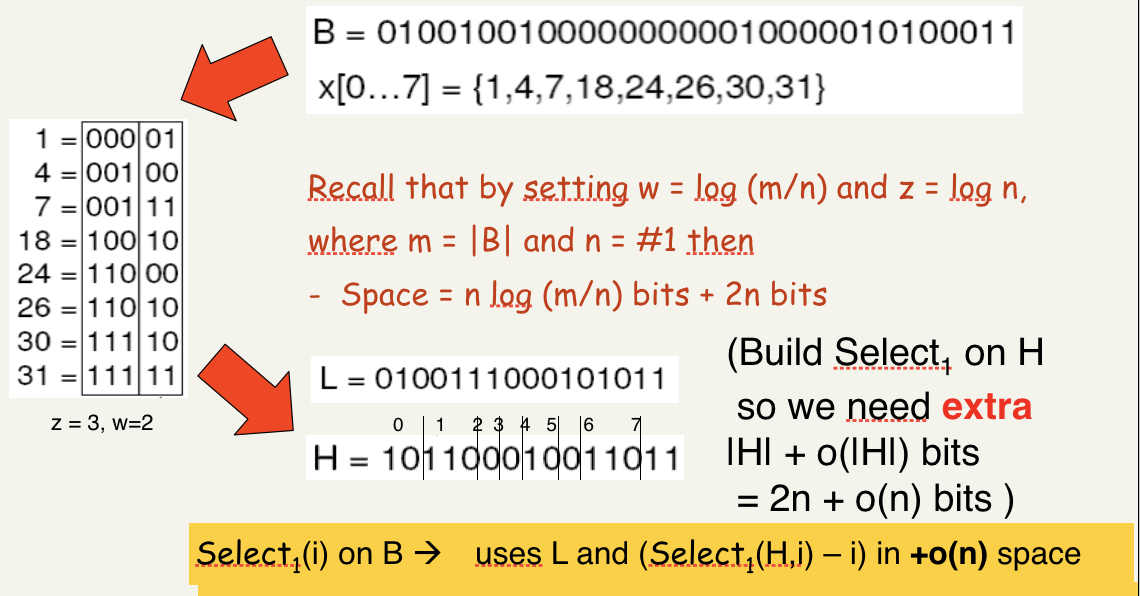
\includegraphics[width=\linewidth]{EliasFanoRankeSelect.png}
  \caption{Slide che spiega come usare Elias Fano come struttura dati per il rank e select}
\end{figure}

Supponiamo di voler trovare 18 che è il 4 numero nella lista. \begin{itemize}
    \item Per prima cosa cerchiamo la quarta coppia di bit in L, in questo caso abbiamo 10.
    \item Poi facciamo $select_1(H,i) - i$. L'operazione di select mi restituisce la posizione dell'i-esimo i in H. In questo caso è 8. A 8 devo sottrarre 4 che è i. Quindi ottengo 4.
    Il quarto 0 che trovo in H, in posizione 7, mi dice che devo vedere la sequenza di 1 successiva, in questo caso abbiamo 10 che mi dice che c'è una sola occorrenza di 100. Quindi abbiamo ricostruito 10010.
\end{itemize}

L'operazioe di Select implementata con Elias Fano richiede quindi uno spazio aggiuntivo di O(n).s


\chapter{Succint Tree}

Per rappresentare un albero binario con la rappresentazione standard abbiamo bisogno di 2 puntatori per ogni nodo, dato che abbiamo n nodi avremo una occupazione in termini di spazio di $2nlogn$ bit. Se poi volessimo aggiungere altre informazioni all'interno dell'albero, come ad esempio un puntatore al padre per ogni nodo, dovremmo andare ad utilizzare altri $nlogn$ bit.

Dato che esistono solamente $2^{2n}$ alberi diversi con n nodi, possiamo andare a differenziarli con soli $2n$ bit.
Quindi esiste un metodo che permette di rappresentare un albero binario con $2n + o(n)$ bit consentendo anche le operazioni basilari in tempo costante (figlio destro, sinistro e padre).


\subsection{Heap Like Notation}

Una possibile soluzione consiste nell'utilizzare una strategia simile a quella che usiamo negli heap.
Questa strategia funziona in questo modo:
\begin{itemize}
    \item Se vogliamo rappresentare l'albero, dobbiamo andare ad aggiungere dei nodi in modo che diventi perfettamente binario. Ogni nodo non foglia dovrà avere 2 figli.
    \item Numeriamo ogni nodo "reale" con 1 e ogni nodo "aggiunto" con lo 0 ottenendo quindi un array che occupa $2n+1$ bit.
    \item Numeriamo poi i nodi presenti all'interno dell'albero in due modi, prima consideriamo solamente i nodi reali e poi anche quelli che invece abbiamo aggiunto. Utilizziamo per la numerazione dei nodi reali altri $n$ bit.
\end{itemize}



  \newcommand{\sep}{\hspace*{.5em}}
  \noindent
  $\fbox{1} \sep \fbox{1} \sep \fbox{1} \sep \fbox{1} \sep \fbox{0} \sep \fbox{1} \sep \fbox{1} \sep \fbox{0} \sep \fbox{1} \sep \fbox{0} \sep \fbox{0} \sep \fbox{1} \sep \fbox{0} \sep \fbox{0} \sep \fbox{0} \sep \fbox{0} \sep \fbox{0}$
  \newline
  \newcommand{\sep}{\hspace*{.5em}}
  \noindent
  $\fbox{\color{red} 1} \sep \fbox{\color{red} 2} \sep \fbox{\color{red} 3} \sep \fbox{\color{red} 4} \sep \fbox{ } \sep \fbox{\color{red} 5} \sep \fbox{\color{red} 6} \sep \fbox{ } \sep \fbox{\color{red} 7} \sep \fbox{ } \sep \fbox{ } \sep \fbox{\color{red} 8} \sep \fbox{ } \sep \fbox{ } \sep \fbox{ } \sep \fbox{ } \sep \fbox{ }$
\newline
  \newcommand{\sep}{\hspace*{.5em}}
  \noindent
  $\fbox{\color{green} 1} \sep \fbox{\color{green} 2} \sep \fbox{\color{green} 3} \sep \fbox{\color{green} 4} \sep \fbox{\color{green}5 } \sep \fbox{\color{green} 6} \sep \fbox{\color{green} 7} \sep \fbox{\color{green} 8} \sep \fbox{\color{green} 9} \sep \fbox{\color{green} 10} \sep \fbox{\color{green} 11} \sep \fbox{\color{green} 12} \sep \fbox{\color{green} 13} \sep \fbox{\color{green} 14} \sep \fbox{\color{green} 15} \sep \fbox{\color{green} 16} \sep \fbox{\color{green} 16}$

Le operazioni sull'albero:

\begin{itemize}
    \item Se voglio il figlio sinistro di un certo nodo $leftChild(K) = 2*K$. Se voglio il figlio destro $rightChild(K) = 2*k + 1$. 
    Ad esempio, se vogliamo il figlio sinistro del nodo 3, $leftChild(3) = 6$ e troviamo la posizione nell'array completo con tutti gli elementi. Guardiamo l'array binario e vediamo che B[6] è uguale a 1 quindi vuol dire che 3 ha un figlio sinistro. Ora dobbiamo trovare la sua posizione reale e il suo valore. Per trovare la sua posizione utilizziamo $rank_1(6)$ ovvero contiamo il numero di 1 che stanno nell'intervallo [1,6] quindi abbiamo che il numero reale è 5.
    Quindi per passare dall'array con la numerazione completa (verde) a quello con la numerazione reale (rosso) si utilizza l'operazione $Rank_1$. Per passare dall'array con la numerazione reale (rosso) a quello con la numerazione completa (verde) si utilizza $Select_1$.
    \item Se vogliamo il padre di un nodo $parent(x) = \lfloor{x/2}\rfloor{}$. In questo caso dobbiamo cercare il parent del nodo considerando la sua posizione nell'array verde, poi la posizione che troviamo fa riferimento all'array rosso ovvero a quello con tutti i nodi "reali".
    Per passare da questa numerazione a quella verde, ovvero per capire la posizione nell'array completo dobbiamo usare $select_1(x)$. Quindi per esempio se cerchiamo $parent(12) = 6$ il 6 fa riferimento all'array rosso. Per trovare la posizione di 6 nell'array completo devo calcolare $select_1(6) = 7$
\end{itemize}

\subsection{Arbitrary Fan-Out: LOUDS}

Si tratta di un altro metodo che possiamo utilizzare per rappresentare un albero binario in modo compresso.
In questo caso sfruttiamo la conoscenza del grado di ogni nodo, dove con grado di un nodo intendiamo il numero dei figli.
Le operazioni supportate con questa rappresentazione sono:

\begin{itemize}
    \item Ricerca del primo figlio di un nodo
    \item Ricerca del fratello di un nodo
    \item Ricerca del padre di un nodo
    \item Calcolo del grado di un nodo
\end{itemize}

La rappresentazione in questo caso è la seguente:

\begin{itemize}
    \item Per ogni nodo calcoliamo il grado del nodo
    \item Numeriamo i nodi in ordine crescente 
    \item Sfruttando la conoscenza del grado dei nodi, scriviamo con la rappresentazione unaria i gradi dei vari nodi per livello. Occupiamo n bit per gli 0 e n bit per gli 1. Va aggiunto un nodo dummy che viene collegato al nodo root.
\end{itemize}



\Tree[.3 [.2 [.0 ]
               [.1 [.0 ]]]
          [.0 ]
                [.3 [.0 ]
                           [.2 [.0 ]
                                [.0 ]
                                       ]
                                       [.2 ]]]

\Tree[.1 [.2 [.5 ]
               [.6 [.10 ]]]
          [.3 ]
                [.4 [.7 ]
                           [.8 [.11 ]
                                [.12 ]
                                       ]
                                       [.9 ]]]

Nella prima figura c'è l'albero con il grado dei nodi segnato su ogni nodo e nella seconda invece c'è la numerazione dei vari nodi.

Le varie operazioni che possiamo fare:

\begin{itemize}
    \item First-Child(k) = $select_0(k)+1$ Ovvero andiamo a trovare la posizione del k-esimo 0 e poi ci sommiamo 1. Questo ci restituisce la posizione del primo figlio del nodo che stiamo cercando.
    Ad esempio $select_0(4) = 11$ ovvero il primo figlio del nodo 4 è in posizione 11 all'interno dell'array binario.
    \item Una volta trovata la posizione del primo figlio, possiamo anche trovare il valore del primo figlio. Per farlo calcoliamo il $rank_1(k)$ ovvero nel sottoarray [0, k] cerchiamo il numero di 1 che mi rappresentano il numero di nodi che sono presenti e restituiamo il numero che troviamo. Questo rappresenta il valore del nodo.
    Continuando l'esempio del primo punto: $rank_1(select_0(4))$ ovvero contiamo il numero di 1 nell'intervallo [0,11] e risulta quindi che il primo figlio di 3 sia il nodo 7.
    \item Il calcolo del next sibling di un certo nodo K avviene in questo modo, consideriamo il valore di A[k+1], se il valore è 0 allora il fratello di k è NULL, altrimenti prendiamo come fratello quello che c'è in A[K+1].
    Ad esempio, abbiamo trovato che il primo figlio di 4 è in posizione 11 $select_0(4) = 11$. Ora dobbiamo andare a vedere dove sta il fratello, allora consideriamo B[$select_0(4)$ + 1]. Se il valore è 0 allora non ha un fratello, se è 1 prendiamo la sua posizione.
    \item Il calcolo del padre di un nodo, dato il nodo K calcoliamo il numero di 0 che troviamo nell'intervallo [0, $select_1(K)$].
    \item Se vogliamo calcolare il grado di un nodo k, usiamo la seguente formula: $select_0(K+1) - select_0(K)$. Troviamo dove inizia e dove finisce il blocco di 1 relativi al nodo K e quindi facciamo la sottrazione per capire quanti 1 ci sono. Il numero di 1 indica anche il numero di figli del nodo K.
\end{itemize}

\chapter{Document Ranking}

\section{Term Frequency and Weighting}

Abbiamo la necessità di ordinare e dare un peso ai documenti che abbiamo nell'inverted index in modo da poter restituire dei risultati migliori nel momento in cui il search engine riceve una query.
Per fare questo possiamo considerare varie metriche per restituire, data una query e l'inverted index i documenti che sono più attinenti rispetto a quello che cerco.
In particolare abbiamo la overlap measure in cui consideriamo solamente l'intersezione tra due vettori binari senza però andare a considerare la lunghezza del documento in cui cerchiamo, la frequenza del termine nel documento e la presenza di parole che sono più comuni di altre, come ad esempio gli articoli. 
Un'altra metrica famosa è la Jaccard Coefficient che è un buon approccio per risolvere questo problema.

Un metodo migliore di quelli già citati è chiamato "tf-idf".
In questo caso, preso un certo termine $t$ e il documento $d$, andiamo a calcolare $tf_{t,d}$ pari al numero di occorrenze del termine t in d.
Poi calcoliamo $idf_t\ =\ log\frac{n}{n_t}$ dove n è il numero completo dei documenti nella collezione mentre $n_t$ è il numero di documenti che contengono il termine t.

Mettendo insieme questi due pesi, otteniamo il peso di ogni parola all'interno dei vari documenti:
$w_{t,d}=tf idf_{t,d} = tf_{t,d} * idf_t$.
La matrice con soli 1 e 0 che rappresenta la presenza di una parola in un certo documento viene quindi trasformata in una matrice di pesi in cui ogni colonna rappresenta il peso dei singoli termini all'interno del documento.
Quindi, presa una query Q e un documento D, lo score del documento d è la somma dei pesi, su tutti i termini della query.

$Score(q,d) = \sum\limits_{t \in q} tfidf_{t,d}$

\section{Vector Space}

Avere una matrice come quella appena descritta ci permette di creare per ogni documento un vettore in cui inseriamo i pesi dei vari termini. Questa rappresentazione dei pesi nella matrice viene chiamato modello Vector Space.
Questi vettori possono essere rappresentati anche sul piano e tra i vari vettori possiamo trovare le somiglianze utilizzando la cosine similarity. Tramite questa misurazione è possibile capire quali sono i documenti che sono maggiormente simili tra loro.

Oltre a confrontare i vettori e quindi i documenti, possiamo anche andare a creare dei nuovi vettori che corrispondono alle query che possiamo fare. Per esempio se abbiamo una query con due termini, creiamo un vettore di N posizioni e mettiamo il valore del peso relativo ai due termini che stiamo cercando. Poi andiamo ad utilizzare la formula della cosine similarity per calcolare la somiglianza tra i vari documenti della matrice e la query.
Lo score quindi viene calcolato in questo modo:
\begin{equation}
    score(q,d)\ =\ \frac{V(q)*V(d)}{|V(q)||V(d)|}
\end{equation}
Lo score equivale alla cosine similarity tra q e d ovvero al coseno dell'angolo che si forma nel piano tra il vettore q e il vettore d.

Questo metodo che consiste nell'utilizzo del vector space e quindi del calcolo delle distanze tra i vettori ha un problema, è facile ingannare il calcolo dello score andando ad inserire all'interno di un documento una certa parola più di una volta in modo da far sembrare che all'interno del documento questa sia davvero ripetuta.
Non è neanche un metodo che scala bene se abbiamo tanti documenti, se invece i documenti sono pochi può essere comunque un buon metodo per iniziare a fare dei confronti.

Volendo implementare il metodo del vector space senza però salvarci in modo esplicito tutta la matrice (visto che sarebbe un enorme spreco di memoria) dobbiamo utilizzare l'inverted index aggiungendo alcune informazioni.
All'interno dell'inverted index, ad ogni docID associamo il valore del $tf_{t,d}$ corrispondente ovvero ci salviamo la frequenza di quella parola all'interno del documento.
Per il calcolo del peso di quella parola nel documento mi serve anche da sapere il numero di documenti in cui la parola compare. Questo lo possiamo salvare sempre nell'inverted index e ci permette quindi di calcolare il peso della parola.

Ora, se abbiamo a disposizione una query che rappresentiamo come un vettore e poi l'inverted index, possiamo usare un algoritmo per calcolare la cosine similarity e trovare i documenti che sono più simili al vettore della query.
Per calcolare la differenza tra la query $q$ e i documenti $d$ possiamo usare la formula generale $cos(q,d) = \sum w_{t,q} * w_{t,d}$.

L'algoritmo poi non fa proprio quello che dice la formula perchè altrimenti sarebbe necessario troppo tempo, quindi l'algoritmo fa la somma degli score dei documenti per ogni termine.


\begin{lstlisting}
CosineScore(q):
    float Scores[N] = 0
    float Length[N]
    for each query term t:
        do calculate w_{t,q} and fetch posting list for t
            for each pair (d, tf_{t,d}) in posting list:
                do Scores[d]+=w_{t,d}*w{t,q}
    Read the array Length
    for each d:
        do Scores[d] = Scores[d]/Length[d]
    return Top K components of Scores[]
\end{lstlisting}

L'algoritmo alloca due array, uno per memorizzare gli score degli N documenti e uno per memorizzare la lunghezza degli N documenti.
Per ogni termine t presente all'interno della query Q calcoliamo il peso $w_{t,q}$ e poi prendiamo la posting list relativa al termine t. 
Per ogni coppia $(d, tf_{t,d})$ presente all'interno della posting list, calcolare $w_{t,d}$ (ovvero calcoliamo il peso del termine t all'interno del documento d) e poi moltiplicarlo per $w_{t_q}$ e sommarlo a Scores[d].
Poi normalizziamo dividendo gli score che troviamo all'interno dell'array per la lunghezza dei documenti.
Arrivati a questo punto nell'array Scores abbiamo gli score dei vari documenti relativi alle parole presenti all'interno della query. 
Dall'array score possiamo estrarre quindi i K componenti (documenti) che sono più vicini alla query.


\section{Approssimare la ricerca dei Top-K Document}

La ricerca dei Top-K documenti risulta essere piuttosto lenta se viene effettuata con la cosine similarity e con il vector Space Model perchè comunque si devono andare a fare molti calcoli.
Quindi una alternativa è approssimare questo calcolo per trovare K documenti che non sono necessariamente i migliori K ma che rappresentano una approssimazione.
Ci sono vari metodi per eseguire questa approssimazione dei Top-K document:

\begin{itemize}
    \item Data una query con q termini, il primo approccio consiste nel considerare per il calcolo dello score solamente quei documenti che contengono almeno un certo numero di termini della query. Spesso si considerano solamente i documenti che contengono almeno (q-1) dei q termini della query.
    In questo modo si scartano tanti documenti e riusciamo a limitare il numero di score da calcolare
    \item Il secondo approccio invece utilizza l'$idf$ dei vari documenti presenti all'interno della posting list. In particolare se questo valore è alto vuol dire che il termine che stiamo cercando è abbastanza raro, al contrario, se l'$idf$ è basso vuol dire che il termine è presente all'interno di quasi tutti i documenti, quindi potrebbe essere un articolo e non c'è necessità di considerare quel termine. Se riusciamo a rimuovere quei termini che sono presenti in tanti documenti andiamo anche a ridurre di molto il numero di documenti di cui va calcolato lo score.
    \item Il terzo approccio è chiamato Champion List. In questo caso abbiamo una fase di pre processing e poi una fase di query. Nella fase di pre processing dobbiamo prendere per ogni termine un numero m di documenti che sono i migliori dal punto di vista dello score tf per quello specifico termine. 
    Una volta scelti gli m elementi per ogni termine abbiamo quindi creato la Champion List. 
    Ora abbiamo la query Q che contiene al suo interno q termini. 
    Prendiamo le champion list dei q termini e le uniamo in un solo set, poi calcoliamo la cosine similarity tra la query e questo set.
    La scelta del numero m di elementi deve essere fatta in modo intelligente, se è troppo piccolo non ha senso e non riusciamo a trovare i top-K document. 
    \item Il quarto approccio è il Fancy-Hits heuristic: in questo caso abbiamo prima una fase di pre processing e poi la query. 
    Nella fase di pre processing andiamo a calcolare per ogni documento il page rank corrispondente. Poi ordiniamo le posting list per PR decrescente e quindi numeriamo in questo modo i vari documenti con ID decrescenti.
    Ora calcoliamo il tf-idf dei vari documenti e dividiamo la posting list in due parti. Nella prima parte, chiamata high, mettiamo M documenti con il tf-idf più alto e nella seconda, low, quelli con tf-idf più basso. Entrambi le parti della posting list sono ordinate per PR decrescente.
    Quando dobbiamo fare la query per prima cosa partiamo dalla parte di posting list high. In questa parte calcoliamo lo score per i vari documenti sommando il valore del PR e del TF-IDF, se riusciamo ad ottenere K top document da inserire all'interno di uno heap allora possiamo terminare, altrimenti dobbiamo passare nella posting list low e continuare a calcolare gli score.
    Quello che possiamo dire, dopo aver diviso in due la posting list è che nella parte high sono presenti tutti documenti che hanno un valore di TF-IDF maggiore di una certa X, quindi nella parte low della posting list avremo i documenti con TF-IDF minore di questa X. Non possiamo dire nulla sul PR, se non che quando prendiamo un certo documento, il PR dei successivi sarà minore di quello precedente, questa relazione però è limitata alle singole posting list, se prendiamo un documento nella posting list high non possiamo dire che il PR sarà maggiore di tutti i documenti della posting list low.
    La scansione si ferma quando abbiamo riempito lo heap con K documenti che sono i top-k documenti.
    Il Page Rank appena nominato può essere un valore compreso tra [0,1], indicato con g(d) che è indipendente dalla query e che indica lo score dei vari documenti.
    Possiamo anche utilizzare questo g(d) in combinazione con le champion list, in questo caso andiamo ad ordinare la posting list non in base al tf-idf più alto ma in base alla somma g(d)+(tf-idf) più alto.
    \item Il quinto approccio è il Clustering: dati N documenti, scegliamo $\sqrt{N}$ documenti e li fissiamo come leader. Poi prendiamo i documenti restanti e calcoliamo la distanza dai leader assegnandoli al leader più vicino.
    I documenti vengono assegnati ad un leader e sono chiamati followers, in media ogni leader avrà $\sqrt{N}$ follower.
    Nel momento in cui abbiamo da fare una query, calcoliamo la distanza tra la query e i vari leader andando a calcolare la cosine similarity. Quando abbiamo trovato il leader più vicino alla query abbiamo anche il set L dei suoi follower, calcoliamo la cosine similarity rispetto ai follower e abbiamo trovato i Top K documenti.
    Questa procedura può variare e possiamo decidere di cercare non soltanto il leader più vicino ma un numero b di leader che sono più vicini alla query, in questo modo abbiamo un numero maggiore di follower e calcoliamo più cosine similarity però approssimiamo meglio i top-k document.
\end{itemize}

\section{Exact Top-K Document}

Dopo aver visto come restituire una approssimazione dei Top K documenti che rispondono ad una query, vediamo come trovare esattamente i K documenti che rispondono ad una certa query.
La strategia più semplice consiste nel trovare i documenti che contengono tutti i termini della query poi successivamente ordiniamo i documenti in base allo score r(d) e restituiamo i primi K risultati.
Una computazione di questo tipo è piuttosto pesante e quindi non riusciamo ad eseguirla velocemente, quindi vorremmo evitare di calcolare lo score di alcuni documenti che siamo sicuri che non finiranno nei top K.

Una tecnica che ci consente di fare questo è la WAND che è un metodo che permette di fare il pruning dei documenti per cui calcolare lo score utilizzando un max heap.
Quando eseguiamo la scansione dei documenti manteniamo un threshold che è il minimo valore contenuto all'interno dello heap, poi quando troviamo un documento che ha uno score maggiore del threshold allora lo inseriamo nel max heap.
Per iterare la lista dei documenti possiamo utilizzare o gli skip Pointer o in alternativa possiamo usare Elias Fano per comprimere la lista e poi navigarla.
Per ogni documento della lista che scorriamo va calcolato uno score che dipende dal documento e dal termine della query che stiamo prendendo in considerazione, $r(t,d)$ = score di t nel documento d.
Per ogni termine della query abbiamo anche un upperbound UB(t) ovvero lo score del documento non supera mai questo upperbound $r(t,d) < UB(t)$.
Per ogni documento lo score complessivo è la somma degli score dei vari termini della query in quel documento. Se abbiamo una query con 3 termini e un documento d:
\newline
\centerline{$score(d) = r(d) = r(t_1,d) + r(t_2,d) + r(t_3,d)$}

L'algoritmo di Wand funziona in questo modo:
\begin{itemize}
    \item Abbiamo le posting list dei vari termini che sono presenti all'interno della query
    \item Ordiniamo le posting list in base al document ID che è puntato in ognuna di esse
    \item Troviamo il pivot, ovvero scorriamo le varie posting list e vediamo se la somma degli upper bound dei vari termini supera il threshold
    \item Quando troviamo una somma di UB che supera il threshold allora prendo l'ultimo termine aggiunto come pivot e considero come non interessanti tutti i documenti precedenti presenti all'interno delle altre posting list.
    
\begin{figure}[h!]
  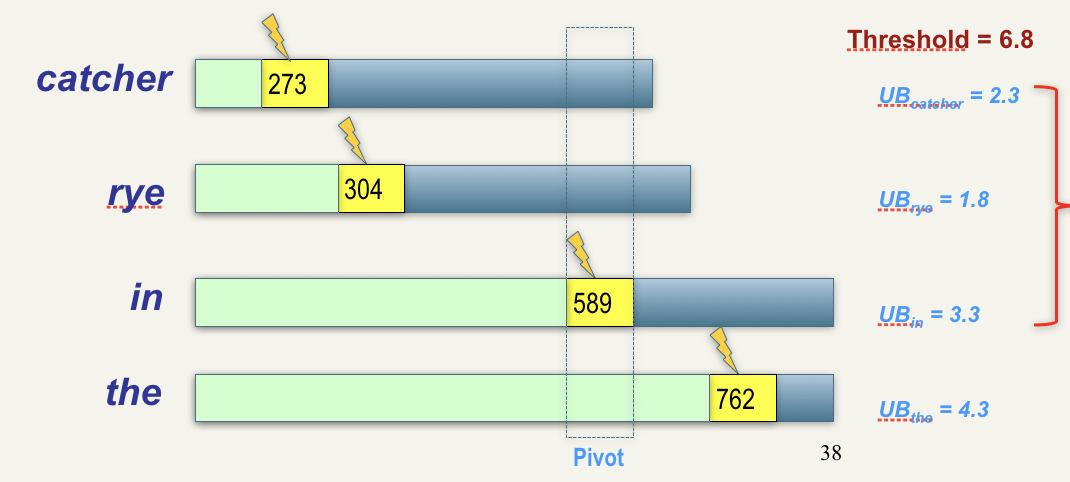
\includegraphics[width=\linewidth]{Wand.png}
  \caption{Scelta del pivot e cancellazione dei precedenti documenti non importanti.}
\end{figure}

    \item Controllo se nelle altre posting list è presente il documento che ha lo stesso ID di quello del pivot. Se è presente allora calcolo lo score di questo documento, altrimenti avanzo al documento successivo. Se lo score di questo documento è maggiore del threshold aggiungo il documento nel maxheap e poi aggiorno anche il threshold.
\end{itemize}

Un problema dell'algoritmo Wand è che quando decidiamo l'upper bound possiamo scegliere un valore che è troppo alto e quindi andiamo a scartare troppo documenti.
Quindi una possibile soluzione è chiamata Blocked Wand, questa soluzione utilizza Wand andando a creare dei blocchi e in ognuno dei blocchi fissa un certo valore per l'upper bound, poi invece di muoverci di documento in documento ci muoviamo di blocco in blocco.
Quando arriviamo in un blocco calcoliamo la somma dei vari upper bound e vediamo se è minore del threshold o no, se è minore allora saltiamo al blocco successivo, altrimenti calcoliamo lo score del documento.

\section{Relevance Feedback}

L'idea del Relevance Feedback consiste nel cercare di utilizzare dei feedback dell'utente nel processo di information retrieval.
In particolare l'utente invia una query poi marca i risultati che vengono restituiti come rilevanti e non rilevanti.
Poi il sistema si adegua al feedback che l'utente ha inviato e cerca di fornire una rappresentazione migliore dei documenti da restituire.
L'operazione di relevance feedback può anche andare avanti per più di una iterazione.

Un algoritmo che possiamo usare per il relevance feedback è l'algoritmo di Rocchio che viene utilizzato per produrre una nuova query che massimizzi la somiglianza con i documenti rilevanti mentre minimizza la somiglianza con i documenti non rilevanti.
Il vettore relativo alla nuova query prodotta dopo l'esecuzione dell'algoritmo lo otteniamo in questo modo:
\newline
\centerline{$q_m = \alpha q_0 + \beta \frac{1}{|D_r|}\sum\limits_{d_j \in D_r} d_j- \gamma\frac{1}{|D_{nr}|}\sum\limits_{d_j \in D_{nr}} d_j$}

Dove $q_m$ è la nuova query, $q_0$ è la vecchia query, $\alpha$ ci permette di decidere come modificare la query originale andando a ridurre la lunghezza del vettore o ad aumentarla, $\beta, \gamma$ sono due valori che usiamo come parametri per decidere a quale termine dare più peso (velocità della convergenza), $D_r$ è l'insieme dei documenti rilevanti e $D_{nr}$ sono i documenti non rilevanti.
Possiamo vedere questa regola anche da un altro punto di vista, prendiamo infatti il vettore q della query e lo mettiamo nel piano, poi con la regola del parallelogramma sommiamo i vettori relativi ai documenti rilevanti mentre sottraiamo i vettori relativi ai documenti non rilevanti.
Trovare $D_r$ e $D_{nr}$ è la parte più importante perchè questo dipende da come il search engine restituisce risultati e dalla qualità di questi risultati.

Oltre al Relevant Feedback è possibile anche utilizzare un tipo differente di Feedback, si tratta dello pseudo relevant feedback che non necessita dell'intervento dell'utente per funzionare.
Ci si basa sulla richiesta dell'utente e sui suoi successivi click, se l'utente clicca sul primo documento vuol dire che l'ha trovato interessante e valido per quella query, se però sta poco nella pagina vuol dire che il documento non era buono, se salta alcuni dei risultati vuol dire che quelli non erano vicini alla query che era stata richiesta.
In questo modo il search engine può adattarsi alle richieste dell'utente senza avere la necessità che l'utente segnali i risultati migliori.

Un altro possibile metodo che ci permette di migliorare la qualità dei risultati di una query è il "Query Expansion".
In questo caso partendo da una certa query, l'utente può andare ad aggiungere dei sinonimi che permettono di eseguire la stessa query oppure possiamo espandere la query andando ad utilizzare dei sinonimi che prendiamo da un Thesauro.
Una alternativa al Thesauro è la global analysis in cui andiamo ad espandere la query utilizzando un grafo che mi rappresenta i log delle query.
Data una certa query creiamo un grafo bipartito in cui colleghiamo le richieste della query ai vari possibili documenti. 
Più utilizziamo il search engine e più il grafo viene espanso e si creano dei cluster di query.

Un'altra possibilità per espandere una query consiste nel creare un Thesauro partendo dai documenti, in particolare andando ad effettuare una analisi delle parole che sono presenti all'interno e cercando di mettere in relazione le parole con il significato del testo e i vari termini anche con le regole grammaticali.

\section{Quality of a search Engine}

Dato un search engine vogliamo essere in grado di capire quanto questo è in grado di restituire risultati in linea con le richieste dell'utente.
Per giudicare la qualità di un search engine tutto ruota attorno alla definizione di rilevante e di non rilevante. Un risultato restituito da un search engine sarà rilevante rispetto alla richiesta se i documenti che vengono mostrati soddisfano le richieste del cliente. Alternativamente sarà non rilevante.
Conoscendo quindi la suddivisione rilevante/non rilevante possiamo considerare un'altra suddivisione tra documenti restituiti in una ricerca e documenti non restituiti.
L'obiettivo del search engine è quello di restituire il più possibile dei documenti che siano rilevanti.
Per analizzare le performance in particolare abbiamo un primo valore che è la Precision P:
\newline
\centerline{$Precision = \frac{#(Documenti\ rilevanti\ restituiti)}{#(Documenti\ restituiti)})$}

Un secondo valore usato per giudicare la qualità del search engine è la Recall R:
\newline
\centerline{$Recall = \frac{#(Documenti\ rilevanti\ restituiti)}{#(Documenti\ rilevanti)}$}

Se creiamo una matrice di confusione fatta in questo modo:

\begin{center}
\begin{tabular}{rcc}
&Relevant&Non Relevant\\
Retrieved&True Positive&False Positive\\
Non Retrieved&False Negative&True Negative\\
\end{tabular}
\end{center}

Possiamo calcolare gli stessi valori di prima in questo modo:
\newline
\centerline{$Precision = \frac{tp}{tp+fp}$}

\newline
\centerline{$Recall = \frac{tp}{tp+fn}$}

Se invece vogliamo utilizzare una singola misurazione per giudicare un search engine possiamo utilizzare la F.
In questo caso la misurazione è la seguente:
\newline
\centerline{$F = \frac{1}{\alpha{\frac{1}{P}+(1-\alpha)\frac{1}{R}}}$}
Dove P è la precion e R la recall, il valore di $\alpha$ invece può valere $\frac{1}{2}$ e in questo caso la misurazione si chiama F1.

Dati due search engine gli umani preferiscono quelli che hanno una precision più alta, se i dati invece vanno dati ad una macchina preferiamo una recall più alta.


\chapter{Link Analysis}

Nel campo dei search engine sta avendo una grande importante l'analisi degli iperlink e della struttura dei grafi. In particolare l'analisi degli iperlink ci permette di dare un giudizio riguardo ad una certa pagina web basandoci sulla quantità di link che puntano a quella determinata pagina. Si tratta in pratica di una misura di centralità per il grafo, i nodi più centrali nel grafo saranno quelli con il maggior numero di link in "entrata".
Con questo sistema sarebbe molto semplice "barare" quindi vengono utilizzati anche altri sistemi per comprendere la centralità di un grafo. In particolare per "barare" e rendere una pagina più centrale mi basterebbe andare a creare tante altre pagine che puntano a quella per cui voglio aumentare lo score. Questo fenomeno è chiamato link spam.

Lo studio degli iper link (anchor text) che mi collegano due pagine ci permette di andare a comprendere molte cose, in particolare, partendo da una pagina A dove troviamo il link che ci porta in B, possiamo dire subito che A approva il contenuto di B dato che lo linka. Inoltre da A possiamo conoscere anche il contenuto della pagina B.

Un anchor text infatti è formato sia dal link sia dalla parola che va cliccata per arrivare alla seconda pagina. In particolare questa parola su cui clicchiamo può essere inserita all'interno di un inverted index e nella sua posting list inseriremo il documento che viene puntato. Ovviamente anche in questo caso va considerato che molti termini saranno piuttosto comuni quando si usa un anchor text, ad esempio "Click" o "Here" non vanno considerati perchè sono molto comuni, invece se trovo la frase "Big Blue" che linka al sito dell'ibm posso considerare questo un link valido e magari nell'inverted index assocerò alla frase "Big Blue" la pagina dell'ibm in modo che quando una persona cerca questo "soprannome" dell'ibm, troverà comunque il link al sito.
Anche in questo caso ci sono stati dei metodi che sono stati utilizzati per permettere l'associazione tra dei link e delle parole. In particolare se tante pagine puntano con un anchor text ad un'altra pagina, è probabile che cercando quella parola esca fuori come primo risultato il link puntato. Questo "attacco" sempre di tipo link spam è stato utilizzato contro Bush perchè erano stati utilizzati degli anchor text con la parola "miserable failure" che puntavano al sito di Bush e quindi cercando su google miserable failure" come primo risultato spuntava il sito di Bush.

\section{Page Rank}

Il page rank è uno dei metodi che vengono utilizzati per dare uno score alle pagine web basandosi sul grafo delle pagine web. In particolare è possibile creare un grafo di internet in cui ogni pagina web è rappresentata con un nodo e poi i link tra le pagine sono gli archi nel grafo.
Quello che succede è che quando si fa una query, vengono presi i documenti interessanti per quella query e si calcola uno score per ognuno dei documenti, poi lo score lo sommiamo ad un altro score che è il page rank.
Il page rank viene calcolato per ogni nodo del grafo ed è un valore che oscilla tra 0 e 1.
L'idea di page rank è che le pagine che vengono visitate maggiormente dagli utenti, vengono considerate più importanti e quindi ottengono uno score più alto. 


\begin{center}
\begin {tikzpicture}[-latex ,auto ,node distance =4 cm and 5cm ,on grid ,
semithick ,
state/.style ={ circle ,top color =white , bottom color = processblue!20 ,
draw,processblue , text=blue , minimum width =1 cm}]
\node[state] (C) {$3$};
\node[state] (A) [above left=of C] {$1$};
\node[state] (B) [above right =of C] {$2$};

\path (C) edge [bend left =25] node[below =0.15 cm] {$1/2$} (A);
\path (A) edge [bend left =25] node[above] {$1$} (B);
\path (C) edge [bend left =15] node[below =0.15 cm] {$1/2$} (B);
\path (B) edge [bend right = -25] node[below =0.15 cm] {$1$} (C);
\end{tikzpicture}
\end{center}

Supponiamo di avere un grafo, possiamo rappresentarlo in una matrice di adiacenza in cui mettiamo nelle varie posizioni 1 se i due nodi sono collegati da un arco e 0 se non sono collegati.

\newline
\begin{center}
\begin{bmatrix}
    0 & 1 & 0 \\
    0 & 0 & 1 \\
    1 & 1 & 0 \\
\end{bmatrix}
\end{center}

Poi partendo da questa matrice possiamo andare a creare la matrice di transazione, detta anche matrice stocastica andando a dividere ogni 1 per il numero di 1 che sono presenti nella riga. Ad esempio nell'ultima riga abbiamo due 1 quindi divido per 2.

\newline
\begin{center}
P = 
\begin{bmatrix}
    0 & 1 & 0 \\
    0 & 0 & 1 \\
    \frac{1}{2} & \frac{1}{2} & 0 \\
\end{bmatrix}
\end{center}

Possiamo rappresentare la distribuzione di probabilità che mostra la posizione nel grafo del "surfer" al momento t come un vettore $\vec{x}$.
Al tempo t=0 avremo il vettore $\vec{x}$ con un solo 1 e tutti gli altri 0, per il tempo 1 dovremo calcolare $\vec{x}_{t=1} = \ve{x}_{t=0}*P$. Al tempo 2 ad esempio dovremo calcolare  $\vec{x}_{t=2} = \ve{x}_{t=1}*P$ che equivale a $\vec{x}_{t=0}*P * P = \ve{x}_{t=0}*P^2$.
In generala la formula per il calcolo della distribuzione della probabilità può essere generalizzata utilizzando un generico tempo $t+1$:
\centerline{$\vec{x}_{t+1}(i) = \vec{x_0}*P^{t+1}$}
\newline
Ovvero consideriamo il vettore di partenza e la matrice di transazione P che viene moltiplicata per se stessa t+1 volte. Per fare questo calcolo viene utilizzato il metodo delle potenze.

Con il random walk arriviamo ad un certo punto in cui la distribuzione di $\vec{x}$ non cambia più da una iterazione alla successiva quindi ci troviamo in una distribuzione stazionaria con $\vec{x}_t$ che diventa quindi lo "steady state distribution", questa distribuzione è chiamata Page Rank.
Questa distribuzione stazionaria, in un grafo fatto bene non dipende dalla distribuzione $\vec{x}_0$ di partenza.
Se abbiamo {$\vec{x}_{t+1}(i) = \vec{x_0}*P^{t+1}$} e $\vec{x}_0$ converge allora vuol dire che:
\begin{equation}
    \vec{x}_{t+1} = \vec{x}_t * P
\end{equation}

\begin{equation}
    \vec{x}_{t+1} = \vec{x}_t
\end{equation}

Sostituiamo la seconda conclusione nella prima e otteniamo:

\begin{equation}
    \vec{x}_{t} = \vec{x}_t * P
\end{equation}

Possiamo riscriverlo aggiungendo un 1 e in questo modo otteniamo:
\begin{equation}
    1 * \vec{x}_{t} = \vec{x}_t * P 
\end{equation}

\begin{equation}
    \vec{x}_t * P = 1 * \vec{x}_{t} 
\end{equation}

Questo vuol dire che $\vec{x}_t$ è l'autovettore sinistro di P e che 1 è il corrispondente autovalore.
Questo succede quando abbiamo la convergenza.

La convergenza e quindi l'esistenza di una distribuzione stazionaria è garantita ed è unica quando il grafo ha due proprietà:
\begin{itemize}
    \item Il grafo deve essere irriducibile ovvero deve essere formato da un'unica componente connessa. Per ogni coppia di nodi del grafo deve esistere un percorso che collega i due nodi.
    \item Il grafo deve essere aperiodico ovvero il massimo comun divisore tra tutte le lunghezze dei cicli presenti all'interno del grafo deve essere 1.
\end{itemize}

Non basta che valga la prima proprietà perchè se non vale anche la seconda abbiamo che la distribuzione dei due nodi cambia ad ogni passaggio e si inverte senza quindi convergere.

Se valgono entrambe le proprietà allora esiste un vettore $\vec{x}_t$ che è l'autovettore di P con autovalore 1 e quindi $\vec{x}_0$ converge.
Se abbiamo la convergenza, il vettore finale $\vec{x}_t$ che otteniamo è la misura di centralità dei vari nodi e rappresenta la probabilità che una certa persona si trovi su un nodo.
Questa distribuzione stazionaria che otteniamo è chiamata page rank.

Come possiamo fare a calcolare questa distribuzione stazionaria?
Dobbiamo approssimare questi valori andando ad eseguire per varie volte il calcolo del vettore $\vec{x}$.
In particolare il grafo completo viene modificato in questo modo, dato un nodo le operazioni che vengono permesse al random surfer sono:
\begin{itemize}
    \item Preso un nodo A in cui mi trovo posso seguire uno degli iperlink e finire in una delle pagine linkate dal nodo A, in particolare le probabilità di seguire gli iperlink presenti nella pagina A sono tutte uguali tra loro.
    \item Operazione telepot: in questo caso ci muoviamo in modo casuale da un nodo presente all'interno del grafo ad un altro nodo o perchè siamo finiti in un nodo che non ha link verso l'esterno o perchè siamo in un nodo e poi ricominciamo la ricerca scrivendo nella barra, senza seguire gli iperlink.
\end{itemize}

L'operazione di Telepot viene effettuata con una probabilità $1-\alpha$ mentre lo spostamento ad un nodo vicino viene effettuato con probabilità $\alpha$.
In questo modo quando ci troviamo in un certo nodo aggiungiamo degli archi che mi collegano agli altri nodi del grafo, la probabilità di questi nodi è $1/N*(1-\alpha)$, le probabilità degli altri archi invece viene scalata di $\alpha$ e quindi le varie probabilità diventano $P*\alpha$.
Avendo aggiunto degli archi e avendo ottenuto un grafo completo, siamo sicuri che il calcolo convergerà.
La scelta della $\alpha$ è importante perchè ci indica quando la struttura del grafo viene considerata nel calcolo del page rank. In particolare con una $\alpha$ bassa, tipo 0 abbiamo che la distribuzione diventa completamente random, un valore molto utilizzato è 0,85 che fornisce una maggiore importanza al grafo e una minore importanza al random jump.

In definitiva, dopo aver introdotto i due tipi di operazioni che possiamo effettuare nel grafo, possiamo definire la formula per il calcolo del page rank.
Nella formula abbiamo un termine che dipende dal teleportation step e un termine che invece indica il contributo del grafo.
\newline
\begin{equation}
    r(i) = \alpha \sum\limits_{j \in B(i)} {\frac{r(j)}{\#out(j)}} + (1-\alpha)\frac{1}{N} 
\end{equation}

La prima parte con la sommatoria indica il contributo che arriva dal grafo, B(i) rappresenta l'insieme dei nodi che puntano a i, la seconda parte invece indica il contributo che arriva dal teleportation step.
Nella sommatoria consideriamo il rank dei nodi che sono vicini del nostro nodo i per cui vogliamo calcolare il rank, il rank viene diviso per il numero di archi che abbiamo in uscita. La sommatoria di questi rank diviso per il numero di archi in uscita viene poi moltiplicata per la $\alpha$. 
Il secondo termine invece è costante durante tutto il calcolo del page rank durante le varie iterazioni.

Il valore del page rank viene poi sommato al TFID per dare importanza alle pagina che devono essere restituite in seguito ad una query effettuata da un utente.

\subsection{Topic Specific Page Rank}

Fino ad ora abbiamo considerato solamente dei grafi in cui, dato un nodo, abbiamo la possibilità di spostarci in un nodo vicino o di saltare ad un altro nodo qualsiasi. Il nodo a cui saltare viene scelto random in base ad una probabilità uniforme.
In alcuni casi vogliamo capire quali pagine sono maggiormente popolari all'interno di un certo set di argomenti, ad esempio vogliamo trovare quali sono le pagine più importanti per quel che riguarda lo sport.

Se consideriamo degli argomenti specifici possiamo adattare il calcolo del ranking delle pagine per l'utente basandoci su quello che l'utente vuole e sui suoi argomenti di maggiore interesse.

Nel classico page rank abbiamo detto che ad ogni step il random walker si trova in un certo nodo e ha una bassa probabilità di fare un salto svolgendo quindi l'operazione di teleportation.
Il teleportation ci porta, nel page rank standard, in una qualsiasi altra pagina del grafo, ogni pagina ha la stessa probabilità di essere la destinazione di un salto.
Nel Topic Specific PageRank invece il random walker può spostarsi solamente in un piccolo set di pagine specifiche, questo set è chiamato "teleport set".
Il set S contiene pagine che sono relative ad un singolo topic, ognuna ha la stessa probabilità di essere raggiunta, per ogni teleport set possiamo calcolare un page rank differente $r_s$.


Se poi l'utente non ha solamente un interesse ma ne ha vari viene creato un vettore in cui le probabilità di saltare ai vari nodi dipendono dalle preferenze dell'utente verso i vari argomenti specifici.

\subsection{Personalized Page Rank}

In questo caso il vettore $\vec{e}$ che viene utilizzato per il teleportation step è formato da tutti 0 e da un solo 1 che corrisponde ad un certo nodo verso il quale tendiamo a tornare. Noi fissiamo un certo nodo e poi calcoliamo la distribuzione di probabilità degli altri nodi del grafo.

In generale, il random walk parte da un certo nodo $i$ del grafo poi si muove verso i vicini del nodo $i$, si allontana un po', poi con probabilità $1-\alpha$ fa un salto e torna indietro al nodo di partenza.
Per ogni nodo $j$ posso calcolare la probabilità che partendo da un nodo $i$ il random walk arrivi nel nodo $j$ e la probabilità è la stessa per tutti i nodi.
Il personalized page rank rappresenta la "relativeness" tra due nodi $i$ e $j$ e ci permette quindi di giudicare la similarità tra i due nodi. Svolgiamo il personalized page rank rispetto ad un certo nodo e troviamo quelli più simili.
Questa probabilità non è simmetrica perchè il grafo è orientato quindi non faccio lo stesso percorso per andare da i a j o per andare da j a i.

La formula del Personalized Page Rank è la seguente:

\newline
\begin{equation}
    p^k(i) = \alpha Ap^{(k-1)}(i) + (1-\alpha)p^{(0)}(i)
\end{equation}

Dove $p^{(0)}(i) = \vec{e}$ dove il vettore $\vec{e}$ è un vettore con tutti 0 tranne un 1 nella posizione i. La formula ci indica che possiamo spostarci nei vicini del nodo i e poi ogni volta con probabilità $1-\alpha$ torniamo al nodo i di partenza.
È importante notare che il valore $p^0(i)$ rimane uguale durante tutti i calcoli del personalized pagerank, devo sempre utilizzare per questo il vettore iniziale delle distribuzioni, quindi avremo sempre un 1 in corrispondenza del nodo a cui saltiamo mentre uno 0 in corrispondenza di tutti gli altri nodi.

Il calcolo del page rank viene utilizzato anche nell'analisi dei social network perchè è un calcolo più robusto rispetto al calcolo dei cammini minimi.

\section{Cosim Rank}

L'obiettivo di Cosim Rank è quello di valutare le somiglianze tra due nodi del grafo senza però andare a considerare tutti gli altri nodi del grafo.
Cosim Rank effettua un random walk partendo dai due nodi e calcola le somiglianze ad ogni step.
Per il calcolo del cosim Rank utilizziamo una modifica della formula del page Rank utilizzata già per il Personalized Pagerank:
\newline
\begin{equation}
    r^{(k)}[i] = \alpha * A * r^{(k-1)} + (1-\alpha) r^{(0)}[i]
\end{equation}

In questa formula nella prima parte abbiamo invertito la matrice A con $r^{(k-1)}$ mentre in page rank è il contrario. 
Ora con questa formula possiamo calcolare il rank dei vari nodi, se però abbiamo due nodi, $i$ e $j$ e vogliamo trovare la probabilità che da questi due nodi si arrivi ad un nodo $x$, rispetto ad $x$ quanto i due nodi devono essere simili?
La relazione tra i, j e x viene misurata con:
\newline
\begin{equation}
    r^{(1)}[I](x) * r^{(1)}[J](x)
\end{equation}
e viene ripetuta per ogni K. Solitamente K si tiene bassa, 2 massimo 3 perchè altrimenti ci allontaniamo troppo dai nodi i e j.

La formula finale del random walker considera la probabilità che un random walker si trovi in un certo nodo dopo un numero limitato K di step:
\newline
\begin{equation}
    S(i,j) = \sum \limits_{K = 0} c^k <r^{(k}[i],r^{(k}[j]>
\end{equation}

Dove $c$ è una costante e l'elevamento alla K serve per attenuare il prodotto scalare, più aumentano le iterazioni, più aumenta la K e quindi più mi allontano da i e da j. Tra le parentesi angolari ci sta il prodotto scalare tra i due rank che ci indica quanto le due distribuzioni sono simili.

Il Cosim rank è simile al Page Rank ma a differenza del Page rank viene svolta una maggiore approssimazione del valore del rank.

\section{HITS: Hypertext Induced Topic Search}

Si tratta di un metodo più che altro teorico perchè non è effettivamente utilizzabile nella pratica a causa del costo computazionale elevato.
A differenza del page rank vogliamo fare in modo che il calcolo dello score delle varie pagine dipenda anche dalla query che l'utente effettua.
Quando viene effettuata una query q, riusciamo a creare due set partendo dalle pagine presenti all'interno del grafo, un set è il root set e contiene quelle pagine che contengono tutte le keyword contenute all'interno della query q. Un secondo set è il base set che invece contiene solamente quelle pagine che sono correlate con quelle del root set senza però contenere direttamente le keyword.

Per ognuna delle pagine che si trovano in questi due set vengono calcolati due score, authority e hub:
\begin{itemize}
    \item Authority score: Per il nodo i calcoliamo a(i), questa a(i) è alta se ci sono tanti nodi che hanno un hub alto e che puntano a i. Quindi se per esempio ad i puntano i nodi j,x,y allora vuol dire che $a(i)\ =\ h(j)\ +\ h(y)\ +\ h(z)$.
    \item Hub score: per il nodo i calcoliamo h(i) che è alto se ci sono nodi che vengono puntati da i e che hanno un authority alta. Quindi se i punta a x,y,z allora vuol dire che $h(i)\ =\ a(x)\ +\ a(y)\ +\ a(z)$.
\end{itemize}

Se vogliamo vederlo in termini di matrici e vettori:
\newline
\begin{equation}
\begin{split}
    \vec{h} = A\vec{a}\\
    \vec{a} = A^T\vec{h}
\end{split}
\end{equation}

Questo perché A è la matrice di adiacenza originale e quindi prendiamo per ogni nodo per cui vogliamo calcolare la hubness una riga di A e per ogni riga i singoli valori (che mi indica i nodi che sono puntati dal nodo i) e poi il corrispondente valore di authority.
Ad esempio, la prima riga di A mi dice che il nodo 1 di cui voglio calcolare l'hubness è collegato al nodo 2. Prendo il valore di authority di 2 e lo moltiplico per 1.

Per calcolare l'authority di un nodo invece devo fare la trasposta della matrice A, in questo modo otteniamo nelle righe i nodi che puntano al nodo i per cui voglio calcolare l'autority. In questo caso prendiamo il valore corrispondente della hubness e poi calcoliamo 1*hubness.       

Possiamo sostituire la prima formula nella seconda e la seconda nella prima:

\begin{equation}
\begin{split}
    \vec{h} = (A*A^T)\vec{h}\\
    \vec{a} = (A^T*A)\vec{a}
\end{split}
\end{equation}

Notiamo che il vettore $\vec{a}$ e il vettore $\vec{h}$ sono gli autovettori per l'autovalore 1 nelle due formule.
Le due matrici sono simmetriche e l'autovalore esiste sempre.
\begin{equation}
\begin{split}
    1*\vec{h} = (A*A^T)\vec{h}\\
    1*\vec{a} = (A^T*A)\vec{a}
\end{split}
\end{equation}

\chapter{LSI}

La matrice relativa all'inverted index con una colonna per documento e una riga per termine è enorme, abbiamo migliaia di documenti e di termini, lavorarci è praticamente impossibile. L'idea di LSI è quella di andare a ridurre la dimensione di questa matrice effettuando delle approssimazioni.

\section{Pre-Processing}

Con LSI gran parte del tempo viene sprecato nella fase di pre processing in cui viene creata la nuova matrice approssimata partendo da quella iniziale. Con questa nuova matrice approssimata poi si procede ad effettuare le query.

Con il metodo classico per vedere la similarità tra due vettori di documenti o tra due vettori di termini svolgiamo i seguenti passi:
\begin{itemize}
    \item Inizialmente partiamo con una matrice A dove $A[i,j]$ rappresenta la frequenza del termine i nel documento j.
    \item Da questa matrice A creiamo una matrice D (dei documenti) che mi rappresenta la similarità tra i vari documenti, dove $D=A^T*A$, se abbiamo n documenti questa matrice sarà di dimensione $n*n$. Usiamo $A^T$ perchè in questo modo sulle righe ci finiscono i vettori dei documenti.
    \item Poi creiamo una seconda matrice, T (per i termini) in cui salviamo la somiglianza tra i termini, ad esempio in posizione $(i,j)$ abbiamo la somiglianza tra il termine $t_i$ e il termine $t_j$. Questa matrice T la calcoliamo come $T=A*A^T$.
\end{itemize}

Dato che vogliamo velocizzare il più possibile la computazione della similarità dobbiamo cercare un metodo alternativo che prevede delle approssimazioni.
Per usare LSI dobbiamo usare un risultato matematico che si chiama SVD.
\newline
Teorema: Data la matrice A di rango r e di dimensione $M*N$, esiste una decomposizione SVD di A nella forma:
\begin{equation}
    A=U*S* V^T
\end{equation}

Dove U è la matrice $M*R$ dove le colonne sono gli autovettori ortonormali della matrice $T=A*A^T$ (Term Matrix) e V è la matrice $N*R$ dove le colonne sono gli autovettori ortonormali della matrice $A^T*A$ (Document Matrix), invece $S$ è una matrice $R*R$ diagonale che contiene gli autovalori di A ordinati in modo decrescente.

Questo teorema mi permette di effettuare la decomposizione della matrice $A$ in $A=U*S*V^T$, U sarà $m*r$, S è $r*r$ e V $r*n$.
Dato che sappiamo che delle r colonne di S solamente k sono piene e non hanno 0, possiamo fare una semplificazione perchè questo ci dice che solamente le prime K colonne di U quando verranno moltiplicate per S avranno un valore diverso da 0 e allo stesso modo solamente le prime K righe di V avranno un valore diverso da 0.
Quindi da qua otteniamo: $U_k$, $S_k$ e $V_k$ e la matrice ridotta e quindi approssimata diveta $A_k = U_k * S_k * V_k$ dove U avrà dimensione $m*k$, S ha dimensione $k*k$ e V ha dimensione $k*n$.
Questa approssimazione $A_k$ di A è la migliore approssimazione di rango K che possiamo creare:
\newline
\begin{equation}
    A_k\ =\ U_k * S_k * V_k^T 
\end{equation}

Rispetto ad $A_k$, $A$ è solamente diversa nel contenuto, ma la dimensione finale è la stessa perchè:
$U_k$ ha dimensione m*k, $S_k$ ha dimensione k*k e $V_k$ ha dimensione k*n. Quindi quando moltiplico le tre matrici alla fine ottengo comunque una matrice m*n.

\section{Approssimare la matrice dei documenti}

Consideriamo la matrice dei documenti D in cui abbiamo le similitudini tra i documenti.
\begin{equation}
    D = A^T*A = (U*S*V)^T*(U*S*V)
\end{equation}

Applichiamo la trasposizione e poi semplifichiamo i due U, S non viene trasposta perchè è diagonale quindi non si sposta nulla dentro alla matrice.

\begin{equation}
    (V*S*U^T)*(U*S*V^T) = (V*S)(S*V^T) = (S*V^T)^T(S*V^T)
\end{equation}

Abbiamo fatto l'ultima modifica per fare in modo di avere lo stesso valore all'interno delle due parentesi, così possiamo sostituirlo con un'altra variabile X.

\begin{equation}
    (S*V^T)^T(S*V^T) = (X)^T(X)
\end{equation}

Questa matrice X può essere ridotta ad una matrice approssimata per il motivo degli zeri spiegato sopra.

\begin{equation}
    (X)^T(X) = (X_k)^T(X_k)
\end{equation}

Quello che vediamo è che A, la matrice iniziale ha lo stesso numero di colonne di $x_k$ mentre invece $x_k$ ha un numero di righe più basso, ovvero $k$ contro le m di A, in ogni caso possiamo rappresentare D in modo approssimato in questo modo:

\begin{equation}
    D = A^T*A \simeq X_k^T*X_k
\end{equation}

Il vantaggio è che mentre in A lavoriamo con un numero di colonne che è O(milioni) in K lavoriamo con un numero di colonne che è O(migliaia), più K è grande e migliore è l'approssimazione.

\section{Rilevare le somiglianze}

Il metodo mostrato sopra è perfetto per controllare se due documenti sono simili.

Mentre all'interno della matrice iniziale A abbiamo una colonna per ogni documento e una riga per ogni termine e poi per ogni elemento della matrice abbiamo la frequenza di quel termine nel documento, nell'approssimazione $x_k$ abbiamo comunque n colonne relative a n documenti ma non abbiamo una riga per termine. Abbiamo solamente k righe con $k<m$ dove m è il numero di righe in A.
Questo è dovuto all'approssimazione, la riduzione del numero di righe mi fa comunque avere una stima della frequenza dei termini nel documento ma mi fa perdere l'associazione precisa tra il termine e la frequenza nel documento. Ogni bucket della matrice in questo caso è chiamato abstract concept. Ci rimane in ogni colonna un set di abstract concept che però non ci permettono di risalire al valore iniziale che avevamo prima di fare la proiezione.
Questo approccio ci fa perdere l'interpretabilità ma comunque viene utilizzato per le performance.

Per ogni termine il vettore di n componenti che avevamo in precedenza viene proiettato in un vettore di K componenti formato da abstract concept dove ogni concept mi indica la rilevanza di quel concept rispetto al termine.
Quindi se ho più di un termine e voglio confrontarli per vedere le similitudini posso andare a vedere il contenuto dei vettori, se moltiplico i vettori e nel risultato trovo un concept c con un valore molto alto vuol dire che il termine è rilevante rispetto a c e quindi i tre concept si riferiscono allo stesso argomento.

\section{Random Projection}

Il random projection è un metodo che scala meglio del precedente, questo metodo si basa sul lemma di Johnson-Linderstrauss. 
Secondo questo lemma:
\begin{itemize}
    \item Abbiamo P punti, ogni punto è un documento
    \item Abbiamo una approssimazione $\epsilon>0$
    \item Abbiamo una funzione f chiamata JL-embedding tale che $f:P->IR^k$
    \item Il lemma mi dice che per ogni coppia di punti u,v vale la proprietà:
    \begin{equation}
        (1 - \epsilon) ||u - v||^2 \leq ||f(u) – f(v)||^2 \leq (1 + \epsilon) ||u-v||^2
    \end{equation}
    Dove il set dei punti P è in realtà il nostro set di documenti e $P->IR^k$ è la proiezione dei punti in K.
\end{itemize}

Più $\epsilon$ è piccola e più è grande K dove $k = O(\epsilon^{-2}logn)$.

Prendo i documenti e cerco di usare il lemma, i documenti che sono vicini tra loro vengono proiettati in punti che sono vicini tra loro.

\chapter{Topic Based Annotators}

Se abbiamo una query e dobbiamo restituire dei documenti associati a questa query, uno dei metodi che abbiamo visto e che si può usare consiste nella cosin similarity. 
Con la cosin similarity prendiamo il vettore della query, i vettori dei vari documenti e calcoliamo il coseno dell'angolo, poi restituiamo i documenti che sono più vicini alla query.
Questo metodo che usa il coseno però non considera i sinonimi e non considera la polisemia. Nel caso dei sinonimi due parole come automobile e macchina non vengono riconosciute come simili anche se il concetto è lo stesso. Nel caso della polisemia invece non si considera il contesto e quindi in questo caso andiamo a considerare identiche due parole che invece hanno un significato differente tra loro, ad esempio stella può essere una stella del cinema ma anche una stella che sta nel cielo.

\section{Soluzione del problema con i grafi}

Il problema è stato risolto nel 2012 da Google che ha introdotto il Knowledge graph, un grafo che contiene nodi e archi in cui i vari nodi sono i documenti mentre gli archi rappresentano i collegamenti e i legami tra i documenti.

Anche Wikipedia ha il suo Knowledge graph in cui ogni nodo rappresenta una pagina e poi da ogni pagina (nodo) siamo collegati a tanti altri nodi grazie alla presenza di anchor text nella pagina. 
Quindi partendo da una certa pagina posso andare a finire in un'altra pagina che è comunque collegata alla mia che stavo visitando.
In Wikipedia c'è anche un grafo Dag che rappresenta le categorie di una pagina di Wikipedia.

\section{Semantic Text Analysis}

Il nuovo approccio che viene utilizzato attualmente per il riconoscimento di informazioni all'interno del testo andando a risolvere i problemi di sinonimi e polisemia consiste nell'andare ad analizzare la frase trovando le parole che possono avere un collegamento con altre pagine. Ogni parola corrisponde ad un argomento e possiamo recuperare le informazioni al riguardo da un database.
Ad esempio, scorro una frase, trovo una parola e vedo se questa può essere un anchor text, se ci sono delle informazioni collegate, la annoto con gli articoli che prendo da Wikipedia.

Eseguendo il parsing del testo riusciamo a differenziare il significato delle parole, per questo motivo riusciamo a risolvere il problema della polysemy andando a mappare una parola verso un certo nodo in base al contesto. Anche il problema dei sinonimi viene risolto perchè le due parole che sono sinonimi andranno ad essere collegate con lo stesso nodo.

In questo caso il problema è che se troviamo un anchor text dobbiamo selezionare solamente le migliori pagine collegate, ne potremmo avere varie ma dobbiamo risolvere questo problema di ambiguità.
Per capire quale sono le pagine migliori collegate ad un certo anchor text abbiamo varie feature che possono essere considerate:
\begin{itemize}
    \item Link Probability: dobbiamo calcolare la probabilità che una certa parola occorra come link all'interno di una pagina. In particolare calcoliamo $P(a)=\frac{frequenza\ di\ a\ come\ anchor}{Frequenza\ di\ a\ nel\ testo}$.
    \item Commonness: calcoliamo la probabilità che un certo anchor text sia collegato ad una certa pagina p. $P(p|a) = \frac{#a\ linked\ to\ p}{#a\ as\ anchor}$. Ovvero se ho 10 link voglio vedere quante volte quell'anchor text mi collega ad una certa pagina specifica p.
    \item Context: considero il contesto attorno alla parola che prendo come anchor text.
    \item Consideriamo alcune feature del grafo, in particolare se abbiamo due pagine e vogliamo vedere se sono simili, non consideriamo solamente se sono collegate tra loro ma andiamo a prendere gli archi entranti in entrambe le pagine e calcoliamo la Jaccard similarity tra questi due set di pagine. Questo score mi indica in modo corretto la similarità tra i due nodi.
\end{itemize}

\section{TagMe}

TagMe è una implementazione delle idee del paragrafo precedente, l'idea è quella di parsare il testo cercando gli anchor text e andando poi a trovare le pagine collegate.
Nella ricerca degli anchor text TagMe cerca sia parola per parola ma anche in base a parole che si trovano vicine, ad esempio trova un nome di una persona e poi il cognome, potrebbero esserci quindi due anchor text, però nome+cognome è un anchor text unico e più grande quindi consideriamo solo questo.
L'obiettivo poi è quello di collegare ogni anchor text ad una sola pagina e quindi ad un solo significato.
Inizialmente le varie parole sono ambigue perchè per ogni anchor text abbiamo più di un collegamento e quindi più di un possibile significato.
Eseguiamo un primo pruning calcolando la commonness per ogni pagina e non considerando quelle pagine che sono una certa soglia.
Per ogni anchor text a abbiamo una serie di pagine Pa associate, dobbiamo trovare le pagine migliori andando a confrontare i vari anchor text e il set di pagine collegate. Ogni valore di un certo set Pa viene confrontato con il valore delle pagine presenti in un set Pb e corrispondente ad un'altra parola.
Lo score delle pagine presenti nei set viene calcolato in questo modo:
\begin{equation}
    vote_b(p_a) = \frac{\sum \limits_{p_b in Pg(b)} rel(p_a, p_b) * Pr(p_b|b)}{|Pg(b)|}
\end{equation}
Alla fine produco uno score e scelgo le pagine con lo score più alto. Poi guardiamo di nuovo la commonness e prendiamo la pagina migliore in base alla commonness.

TagMe può avere un problema, si possono infatti creare dei cluster di possibili pagine migliori per un certo anchor text in cui la distanza tra le varie pagine è molto bassa e quindi non c'è effettivamente una pagina con uno score alto che spicca su tutte le altre. In questo caso non si riesce a disambiguare bene.

Nonostante l'esistenza di TagMe, tf-idf rimane comunque una possibile soluzione al problema della ricerca delle somiglianze perchè in alcuni casi TagMe non è in grado di trovare le entity all'interno del testo e quindi non riconosce alcune parole come anchor text.


\end{document}
